\documentclass[twoside]{book}

% Packages required by doxygen
\usepackage{calc}
\usepackage{doxygen}
\usepackage{graphicx}
\usepackage[utf8]{inputenc}
\usepackage{makeidx}
\usepackage{multicol}
\usepackage{multirow}
\usepackage{textcomp}
\usepackage[table]{xcolor}

% Font selection
\usepackage[T1]{fontenc}
\usepackage{mathptmx}
\usepackage[scaled=.90]{helvet}
\usepackage{courier}
\usepackage{amssymb}
\usepackage{sectsty}
\renewcommand{\familydefault}{\sfdefault}
\allsectionsfont{%
  \fontseries{bc}\selectfont%
  \color{darkgray}%
}
\renewcommand{\DoxyLabelFont}{%
  \fontseries{bc}\selectfont%
  \color{darkgray}%
}

% Page & text layout
\usepackage{geometry}
\geometry{%
  a4paper,%
  top=2.5cm,%
  bottom=2.5cm,%
  left=2.5cm,%
  right=2.5cm%
}
\tolerance=750
\hfuzz=15pt
\hbadness=750
\setlength{\emergencystretch}{15pt}
\setlength{\parindent}{0cm}
\setlength{\parskip}{0.2cm}
\makeatletter
\renewcommand{\paragraph}{%
  \@startsection{paragraph}{4}{0ex}{-1.0ex}{1.0ex}{%
    \normalfont\normalsize\bfseries\SS@parafont%
  }%
}
\renewcommand{\subparagraph}{%
  \@startsection{subparagraph}{5}{0ex}{-1.0ex}{1.0ex}{%
    \normalfont\normalsize\bfseries\SS@subparafont%
  }%
}
\makeatother

% Headers & footers
\usepackage{fancyhdr}
\pagestyle{fancyplain}
\fancyhead[LE]{\fancyplain{}{\bfseries\thepage}}
\fancyhead[CE]{\fancyplain{}{}}
\fancyhead[RE]{\fancyplain{}{\bfseries\leftmark}}
\fancyhead[LO]{\fancyplain{}{\bfseries\rightmark}}
\fancyhead[CO]{\fancyplain{}{}}
\fancyhead[RO]{\fancyplain{}{\bfseries\thepage}}
\fancyfoot[LE]{\fancyplain{}{}}
\fancyfoot[CE]{\fancyplain{}{}}
\fancyfoot[RE]{\fancyplain{}{\bfseries\scriptsize Generated on Sun Mar 6 2016 13\-:33\-:53 for Battle\-Ship2\-D by Doxygen }}
\fancyfoot[LO]{\fancyplain{}{\bfseries\scriptsize Generated on Sun Mar 6 2016 13\-:33\-:53 for Battle\-Ship2\-D by Doxygen }}
\fancyfoot[CO]{\fancyplain{}{}}
\fancyfoot[RO]{\fancyplain{}{}}
\renewcommand{\footrulewidth}{0.4pt}
\renewcommand{\chaptermark}[1]{%
  \markboth{#1}{}%
}
\renewcommand{\sectionmark}[1]{%
  \markright{\thesection\ #1}%
}

% Indices & bibliography
\usepackage{natbib}
\usepackage[titles]{tocloft}
\setcounter{tocdepth}{3}
\setcounter{secnumdepth}{5}
\makeindex

% Hyperlinks (required, but should be loaded last)
\usepackage{ifpdf}
\ifpdf
  \usepackage[pdftex,pagebackref=true]{hyperref}
\else
  \usepackage[ps2pdf,pagebackref=true]{hyperref}
\fi
\hypersetup{%
  colorlinks=true,%
  linkcolor=blue,%
  citecolor=blue,%
  unicode%
}

% Custom commands
\newcommand{\clearemptydoublepage}{%
  \newpage{\pagestyle{empty}\cleardoublepage}%
}


%===== C O N T E N T S =====

\begin{document}

% Titlepage & ToC
\hypersetup{pageanchor=false}
\pagenumbering{roman}
\begin{titlepage}
\vspace*{7cm}
\begin{center}%
{\Large Battle\-Ship2\-D \\[1ex]\large 1 }\\
\vspace*{1cm}
{\large Generated by Doxygen 1.8.6}\\
\vspace*{0.5cm}
{\small Sun Mar 6 2016 13:33:53}\\
\end{center}
\end{titlepage}
\clearemptydoublepage
\tableofcontents
\clearemptydoublepage
\pagenumbering{arabic}
\hypersetup{pageanchor=true}

%--- Begin generated contents ---
\chapter{Namespace Index}
\section{Packages}
Here are the packages with brief descriptions (if available)\-:\begin{DoxyCompactList}
\item\contentsline{section}{\hyperlink{namespacebattleship2D}{battleship2\-D} }{\pageref{namespacebattleship2D}}{}
\item\contentsline{section}{\hyperlink{namespacebattleship2D_1_1model}{battleship2\-D.\-model} }{\pageref{namespacebattleship2D_1_1model}}{}
\end{DoxyCompactList}

\chapter{Class Index}
\section{Class List}
Here are the classes, structs, unions and interfaces with brief descriptions\-:\begin{DoxyCompactList}
\item\contentsline{section}{\hyperlink{classbattleship2D_1_1model_1_1BoardModel}{battleship2\-D.\-model.\-Board\-Model} \\*Global board for manipulating cells }{\pageref{classbattleship2D_1_1model_1_1BoardModel}}{}
\item\contentsline{section}{\hyperlink{classbattleship2D_1_1model_1_1CellModel}{battleship2\-D.\-model.\-Cell\-Model} \\*Board model element }{\pageref{classbattleship2D_1_1model_1_1CellModel}}{}
\item\contentsline{section}{\hyperlink{enumbattleship2D_1_1model_1_1CellType}{battleship2\-D.\-model.\-Cell\-Type} \\*Cell Types }{\pageref{enumbattleship2D_1_1model_1_1CellType}}{}
\item\contentsline{section}{\hyperlink{classbattleship2D_1_1model_1_1Coord2D}{battleship2\-D.\-model.\-Coord2\-D} \\*(row,column) -\/ coordinates pair inside a 2\-D array }{\pageref{classbattleship2D_1_1model_1_1Coord2D}}{}
\item\contentsline{section}{\hyperlink{enumbattleship2D_1_1model_1_1Direction}{battleship2\-D.\-model.\-Direction} \\*Directions along which ships are placed }{\pageref{enumbattleship2D_1_1model_1_1Direction}}{}
\item\contentsline{section}{\hyperlink{classbattleship2D_1_1model_1_1Fleet}{battleship2\-D.\-model.\-Fleet} \\*\hyperlink{classbattleship2D_1_1model_1_1Fleet}{Fleet} of Ships }{\pageref{classbattleship2D_1_1model_1_1Fleet}}{}
\item\contentsline{section}{\hyperlink{classbattleship2D_1_1model_1_1Ship}{battleship2\-D.\-model.\-Ship} \\*\hyperlink{classbattleship2D_1_1model_1_1Ship}{Ship} representation on the board A ship is made of tiles aligned along either the X-\/axis or the Y-\/axis }{\pageref{classbattleship2D_1_1model_1_1Ship}}{}
\item\contentsline{section}{\hyperlink{enumbattleship2D_1_1model_1_1ShipType}{battleship2\-D.\-model.\-Ship\-Type} \\*\hyperlink{classbattleship2D_1_1model_1_1Ship}{Ship} types }{\pageref{enumbattleship2D_1_1model_1_1ShipType}}{}
\item\contentsline{section}{\hyperlink{enumbattleship2D_1_1model_1_1SkillLevel}{battleship2\-D.\-model.\-Skill\-Level} \\*Determines the computer skill level }{\pageref{enumbattleship2D_1_1model_1_1SkillLevel}}{}
\item\contentsline{section}{\hyperlink{enumbattleship2D_1_1model_1_1Turn}{battleship2\-D.\-model.\-Turn} \\*Determines players turn }{\pageref{enumbattleship2D_1_1model_1_1Turn}}{}
\end{DoxyCompactList}

\chapter{File Index}
\section{File List}
Here is a list of all files with brief descriptions\-:\begin{DoxyCompactList}
\item\contentsline{section}{/home/xaviator/\-Enseignements/2015-\/2016/\-S\-F\-A/\-M1-\/\-Info/\-I\-H\-M/\-Battle\-Ship2\-D\-\_\-students/battleship2\-D/model/\hyperlink{BoardModel_8java}{Board\-Model.\-java} }{\pageref{BoardModel_8java}}{}
\item\contentsline{section}{/home/xaviator/\-Enseignements/2015-\/2016/\-S\-F\-A/\-M1-\/\-Info/\-I\-H\-M/\-Battle\-Ship2\-D\-\_\-students/battleship2\-D/model/\hyperlink{CellModel_8java}{Cell\-Model.\-java} }{\pageref{CellModel_8java}}{}
\item\contentsline{section}{/home/xaviator/\-Enseignements/2015-\/2016/\-S\-F\-A/\-M1-\/\-Info/\-I\-H\-M/\-Battle\-Ship2\-D\-\_\-students/battleship2\-D/model/\hyperlink{CellType_8java}{Cell\-Type.\-java} }{\pageref{CellType_8java}}{}
\item\contentsline{section}{/home/xaviator/\-Enseignements/2015-\/2016/\-S\-F\-A/\-M1-\/\-Info/\-I\-H\-M/\-Battle\-Ship2\-D\-\_\-students/battleship2\-D/model/\hyperlink{Coord2D_8java}{Coord2\-D.\-java} }{\pageref{Coord2D_8java}}{}
\item\contentsline{section}{/home/xaviator/\-Enseignements/2015-\/2016/\-S\-F\-A/\-M1-\/\-Info/\-I\-H\-M/\-Battle\-Ship2\-D\-\_\-students/battleship2\-D/model/\hyperlink{Direction_8java}{Direction.\-java} }{\pageref{Direction_8java}}{}
\item\contentsline{section}{/home/xaviator/\-Enseignements/2015-\/2016/\-S\-F\-A/\-M1-\/\-Info/\-I\-H\-M/\-Battle\-Ship2\-D\-\_\-students/battleship2\-D/model/\hyperlink{Fleet_8java}{Fleet.\-java} }{\pageref{Fleet_8java}}{}
\item\contentsline{section}{/home/xaviator/\-Enseignements/2015-\/2016/\-S\-F\-A/\-M1-\/\-Info/\-I\-H\-M/\-Battle\-Ship2\-D\-\_\-students/battleship2\-D/model/\hyperlink{Ship_8java}{Ship.\-java} }{\pageref{Ship_8java}}{}
\item\contentsline{section}{/home/xaviator/\-Enseignements/2015-\/2016/\-S\-F\-A/\-M1-\/\-Info/\-I\-H\-M/\-Battle\-Ship2\-D\-\_\-students/battleship2\-D/model/\hyperlink{ShipType_8java}{Ship\-Type.\-java} }{\pageref{ShipType_8java}}{}
\item\contentsline{section}{/home/xaviator/\-Enseignements/2015-\/2016/\-S\-F\-A/\-M1-\/\-Info/\-I\-H\-M/\-Battle\-Ship2\-D\-\_\-students/battleship2\-D/model/\hyperlink{SkillLevel_8java}{Skill\-Level.\-java} }{\pageref{SkillLevel_8java}}{}
\item\contentsline{section}{/home/xaviator/\-Enseignements/2015-\/2016/\-S\-F\-A/\-M1-\/\-Info/\-I\-H\-M/\-Battle\-Ship2\-D\-\_\-students/battleship2\-D/model/\hyperlink{Turn_8java}{Turn.\-java} }{\pageref{Turn_8java}}{}
\end{DoxyCompactList}

\chapter{Namespace Documentation}
\hypertarget{namespacebattleship2D}{\section{Package battleship2\-D}
\label{namespacebattleship2D}\index{battleship2\-D@{battleship2\-D}}
}
\subsection*{Packages}
\begin{DoxyCompactItemize}
\item 
package \hyperlink{namespacebattleship2D_1_1model}{model}
\end{DoxyCompactItemize}

\hypertarget{namespacebattleship2D_1_1model}{\section{Package battleship2\-D.\-model}
\label{namespacebattleship2D_1_1model}\index{battleship2\-D.\-model@{battleship2\-D.\-model}}
}
\subsection*{Classes}
\begin{DoxyCompactItemize}
\item 
class \hyperlink{classbattleship2D_1_1model_1_1BoardModel}{Board\-Model}
\begin{DoxyCompactList}\small\item\em Global board for manipulating cells. \end{DoxyCompactList}\item 
class \hyperlink{classbattleship2D_1_1model_1_1CellModel}{Cell\-Model}
\begin{DoxyCompactList}\small\item\em Board model element. \end{DoxyCompactList}\item 
enum \hyperlink{enumbattleship2D_1_1model_1_1CellType}{Cell\-Type}
\begin{DoxyCompactList}\small\item\em Cell Types. \end{DoxyCompactList}\item 
class \hyperlink{classbattleship2D_1_1model_1_1Coord2D}{Coord2\-D}
\begin{DoxyCompactList}\small\item\em (row,column) -\/ coordinates pair inside a 2\-D array \end{DoxyCompactList}\item 
enum \hyperlink{enumbattleship2D_1_1model_1_1Direction}{Direction}
\begin{DoxyCompactList}\small\item\em Directions along which ships are placed. \end{DoxyCompactList}\item 
class \hyperlink{classbattleship2D_1_1model_1_1Fleet}{Fleet}
\begin{DoxyCompactList}\small\item\em \hyperlink{classbattleship2D_1_1model_1_1Fleet}{Fleet} of Ships. \end{DoxyCompactList}\item 
class \hyperlink{classbattleship2D_1_1model_1_1Ship}{Ship}
\begin{DoxyCompactList}\small\item\em \hyperlink{classbattleship2D_1_1model_1_1Ship}{Ship} representation on the board A ship is made of tiles aligned along either the X-\/axis or the Y-\/axis. \end{DoxyCompactList}\item 
enum \hyperlink{enumbattleship2D_1_1model_1_1ShipType}{Ship\-Type}
\begin{DoxyCompactList}\small\item\em \hyperlink{classbattleship2D_1_1model_1_1Ship}{Ship} types. \end{DoxyCompactList}\item 
enum \hyperlink{enumbattleship2D_1_1model_1_1SkillLevel}{Skill\-Level}
\begin{DoxyCompactList}\small\item\em Determines the computer skill level. \end{DoxyCompactList}\item 
enum \hyperlink{enumbattleship2D_1_1model_1_1Turn}{Turn}
\begin{DoxyCompactList}\small\item\em Determines players turn. \end{DoxyCompactList}\end{DoxyCompactItemize}

\chapter{Class Documentation}
\hypertarget{classbattleship2D_1_1model_1_1BoardModel}{\section{battleship2\-D.\-model.\-Board\-Model Class Reference}
\label{classbattleship2D_1_1model_1_1BoardModel}\index{battleship2\-D.\-model.\-Board\-Model@{battleship2\-D.\-model.\-Board\-Model}}
}


Global board for manipulating cells.  




Collaboration diagram for battleship2\-D.\-model.\-Board\-Model\-:\nopagebreak
\begin{figure}[H]
\begin{center}
\leavevmode
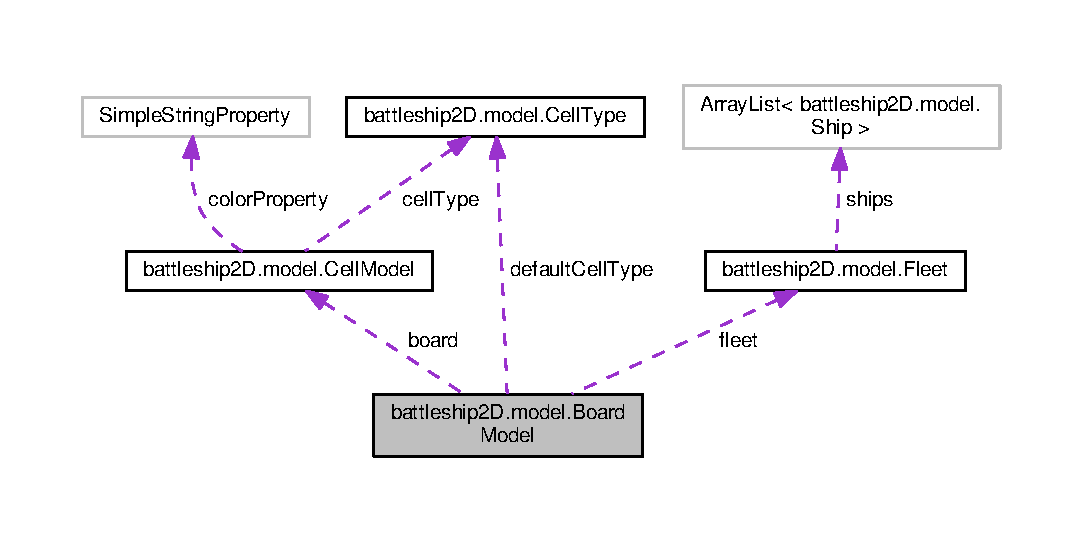
\includegraphics[width=350pt]{classbattleship2D_1_1model_1_1BoardModel__coll__graph}
\end{center}
\end{figure}
\subsection*{Public Member Functions}
\begin{DoxyCompactItemize}
\item 
\hyperlink{classbattleship2D_1_1model_1_1BoardModel_ae4cfe2d64ce4aced2bd0ae0efd42764e}{Board\-Model} (\hyperlink{enumbattleship2D_1_1model_1_1CellType}{Cell\-Type} cell\-Type)
\begin{DoxyCompactList}\small\item\em Constructor. \end{DoxyCompactList}\item 
\hyperlink{classbattleship2D_1_1model_1_1CellModel}{Cell\-Model} \hyperlink{classbattleship2D_1_1model_1_1BoardModel_a301ebd2b0d375366c4c2549988c70522}{adjacent\-Cell} (\hyperlink{classbattleship2D_1_1model_1_1CellModel}{Cell\-Model} cell\-Model, \hyperlink{enumbattleship2D_1_1model_1_1Direction}{Direction} direction)
\begin{DoxyCompactList}\small\item\em Searches for the cells adjacent to another along cardinal directions. \end{DoxyCompactList}\item 
\hyperlink{classbattleship2D_1_1model_1_1CellModel}{Cell\-Model} \hyperlink{classbattleship2D_1_1model_1_1BoardModel_a5127bef6a246972c2cdacc38a07b36d8}{adjacent\-Cell} (\hyperlink{classbattleship2D_1_1model_1_1CellModel}{Cell\-Model} cell\-Model, \hyperlink{enumbattleship2D_1_1model_1_1Direction}{Direction} direction, int step)
\begin{DoxyCompactList}\small\item\em Searches for the cells adjacent to another along cardinal directions. \end{DoxyCompactList}\item 
\hyperlink{classbattleship2D_1_1model_1_1Coord2D}{Coord2\-D} \hyperlink{classbattleship2D_1_1model_1_1BoardModel_a9f192bbde7b6523a8ec7e78e09f08db1}{cell\-Coords} (\hyperlink{classbattleship2D_1_1model_1_1CellModel}{Cell\-Model} cell\-Model)
\item 
void \hyperlink{classbattleship2D_1_1model_1_1BoardModel_a70d5de35696401c7271e63e7392da0a0}{display} ()
\begin{DoxyCompactList}\small\item\em Displays board's contents. \end{DoxyCompactList}\item 
\hyperlink{classbattleship2D_1_1model_1_1CellModel}{Cell\-Model} \hyperlink{classbattleship2D_1_1model_1_1BoardModel_a91ddb22e8123ffd145fc5c05585110f8}{find\-First\-Cell\-Of\-Type} (\hyperlink{enumbattleship2D_1_1model_1_1CellType}{Cell\-Type} cell\-Type)
\item 
Boolean \hyperlink{classbattleship2D_1_1model_1_1BoardModel_a4a79e7a8f51182ced9478fee68f7842a}{is\-Cell\-Of\-Type} (\hyperlink{classbattleship2D_1_1model_1_1CellModel}{Cell\-Model} cell\-Model, \hyperlink{enumbattleship2D_1_1model_1_1CellType}{Cell\-Type} cell\-Type)
\begin{DoxyCompactList}\small\item\em Checks whether a cell is of a given type. \end{DoxyCompactList}\item 
Boolean \hyperlink{classbattleship2D_1_1model_1_1BoardModel_a3a7275142b51bcf384bc40c8836038e4}{is\-Cell\-Type\-Inside} (\hyperlink{enumbattleship2D_1_1model_1_1CellType}{Cell\-Type} cell\-Type)
\item 
\hyperlink{classbattleship2D_1_1model_1_1CellModel}{Cell\-Model} \hyperlink{classbattleship2D_1_1model_1_1BoardModel_a528b0e9bf9dbd8cfd0f9f3754cea5d79}{random\-Cell} (\hyperlink{enumbattleship2D_1_1model_1_1CellType}{Cell\-Type} cell\-Type, Boolean is\-Cell\-Type)
\item 
void \hyperlink{classbattleship2D_1_1model_1_1BoardModel_a28b2129ced4821bddf7a3c5e27bfbf8e}{replace\-All} (\hyperlink{enumbattleship2D_1_1model_1_1CellType}{Cell\-Type} old\-Cell\-Type, \hyperlink{enumbattleship2D_1_1model_1_1CellType}{Cell\-Type} new\-Cell\-Type)
\begin{DoxyCompactList}\small\item\em Replaces a set of cell types with another one. \end{DoxyCompactList}\item 
void \hyperlink{classbattleship2D_1_1model_1_1BoardModel_a7aa5da807e5e13cd066ff43096c0f159}{reset} (\hyperlink{enumbattleship2D_1_1model_1_1CellType}{Cell\-Type} cell\-Type)
\begin{DoxyCompactList}\small\item\em Resets board's contents to default value. \end{DoxyCompactList}\item 
\hyperlink{classbattleship2D_1_1model_1_1CellModel}{Cell\-Model} \hyperlink{classbattleship2D_1_1model_1_1BoardModel_afa03fdf7f571196dcf71d6dd6026f5c2}{get\-Cell\-Model} (int row, int column)
\item 
\hyperlink{enumbattleship2D_1_1model_1_1CellType}{Cell\-Type} \hyperlink{classbattleship2D_1_1model_1_1BoardModel_accfa1eebdda7de04ac59c2399d27eeef}{get\-Default\-Cell\-Type} ()
\item 
\hyperlink{classbattleship2D_1_1model_1_1Fleet}{Fleet} \hyperlink{classbattleship2D_1_1model_1_1BoardModel_a4071154c05caa46d691892f565ff9aeb}{get\-Fleet} ()
\end{DoxyCompactItemize}
\subsection*{Static Public Member Functions}
\begin{DoxyCompactItemize}
\item 
static boolean \hyperlink{classbattleship2D_1_1model_1_1BoardModel_a96c8e6db76df3433972e99d4d2ebada0}{are\-All\-Cells\-Of\-Type} (Array\-List$<$ \hyperlink{classbattleship2D_1_1model_1_1CellModel}{Cell\-Model} $>$cell\-Models, \hyperlink{enumbattleship2D_1_1model_1_1CellType}{Cell\-Type} cell\-Type)
\item 
static \hyperlink{classbattleship2D_1_1model_1_1CellModel}{Cell\-Model} \hyperlink{classbattleship2D_1_1model_1_1BoardModel_ab82fdc92af2604db0677e050632e4c52}{find\-First\-Cell\-Of\-Type} (Array\-List$<$ \hyperlink{classbattleship2D_1_1model_1_1CellModel}{Cell\-Model} $>$cell\-Models, \hyperlink{enumbattleship2D_1_1model_1_1CellType}{Cell\-Type} cell\-Type)
\begin{DoxyCompactList}\small\item\em Determine whether there is at least one element of a cell set with a given type. \end{DoxyCompactList}\end{DoxyCompactItemize}
\subsection*{Static Public Attributes}
\begin{DoxyCompactItemize}
\item 
static int \hyperlink{classbattleship2D_1_1model_1_1BoardModel_ae460f6b5b6c201a4260f504cee2bbe88}{B\-O\-A\-R\-D\-\_\-\-S\-I\-Z\-E} = 10
\begin{DoxyCompactList}\small\item\em Game board size. \end{DoxyCompactList}\end{DoxyCompactItemize}
\subsection*{Protected Attributes}
\begin{DoxyCompactItemize}
\item 
final \hyperlink{classbattleship2D_1_1model_1_1CellModel}{Cell\-Model}\mbox{[}$\,$\mbox{]}\mbox{[}$\,$\mbox{]} \hyperlink{classbattleship2D_1_1model_1_1BoardModel_aef391200a2e699e06c2f0efa9c75f93b}{board}
\begin{DoxyCompactList}\small\item\em 2\-D board \end{DoxyCompactList}\item 
final \hyperlink{classbattleship2D_1_1model_1_1Fleet}{Fleet} \hyperlink{classbattleship2D_1_1model_1_1BoardModel_a31a41118d87b809557a0d3579068efe9}{fleet}
\begin{DoxyCompactList}\small\item\em \hyperlink{classbattleship2D_1_1model_1_1Fleet}{Fleet} of ships to place on the board. \end{DoxyCompactList}\end{DoxyCompactItemize}
\subsection*{Private Member Functions}
\begin{DoxyCompactItemize}
\item 
Boolean \hyperlink{classbattleship2D_1_1model_1_1BoardModel_a834c3bb01a7486857faab326f2c9af33}{are\-Coordinates\-Inside} (int row, int column)
\begin{DoxyCompactList}\small\item\em Checks whether a pair of coordinates is located inside the board. \end{DoxyCompactList}\item 
\hyperlink{classbattleship2D_1_1model_1_1CellModel}{Cell\-Model} \hyperlink{classbattleship2D_1_1model_1_1BoardModel_a84e362612177e2e6b989713bc5fff49f}{find\-Cell\-With\-Id} (Integer \hyperlink{classbattleship2D_1_1model_1_1BoardModel_a6a039e078208c6fe2df015b9b3e6bdf1}{cell\-Id})
\begin{DoxyCompactList}\small\item\em Searches for a cell, knowing its id. \end{DoxyCompactList}\item 
void \hyperlink{classbattleship2D_1_1model_1_1BoardModel_a3e3f9d28be068d3ec4f56be1e4fa4258}{init} (\hyperlink{enumbattleship2D_1_1model_1_1CellType}{Cell\-Type} cell\-Type)
\begin{DoxyCompactList}\small\item\em Initializes board's contents. \end{DoxyCompactList}\end{DoxyCompactItemize}
\subsection*{Private Attributes}
\begin{DoxyCompactItemize}
\item 
Integer \hyperlink{classbattleship2D_1_1model_1_1BoardModel_a6a039e078208c6fe2df015b9b3e6bdf1}{cell\-Id}
\begin{DoxyCompactList}\small\item\em Cell identifier. \end{DoxyCompactList}\item 
final \hyperlink{enumbattleship2D_1_1model_1_1CellType}{Cell\-Type} \hyperlink{classbattleship2D_1_1model_1_1BoardModel_a0b9c7c69532e0643f423711e0e5f478e}{default\-Cell\-Type}
\begin{DoxyCompactList}\small\item\em Default cell type for board cells. \end{DoxyCompactList}\end{DoxyCompactItemize}


\subsection{Detailed Description}
Global board for manipulating cells. 

\begin{DoxyAuthor}{Author}
xaviator 
\end{DoxyAuthor}


\subsection{Constructor \& Destructor Documentation}
\hypertarget{classbattleship2D_1_1model_1_1BoardModel_ae4cfe2d64ce4aced2bd0ae0efd42764e}{\index{battleship2\-D\-::model\-::\-Board\-Model@{battleship2\-D\-::model\-::\-Board\-Model}!Board\-Model@{Board\-Model}}
\index{Board\-Model@{Board\-Model}!battleship2D::model::BoardModel@{battleship2\-D\-::model\-::\-Board\-Model}}
\subsubsection[{Board\-Model}]{\setlength{\rightskip}{0pt plus 5cm}battleship2\-D.\-model.\-Board\-Model.\-Board\-Model (
\begin{DoxyParamCaption}
\item[{{\bf Cell\-Type}}]{cell\-Type}
\end{DoxyParamCaption}
)}}\label{classbattleship2D_1_1model_1_1BoardModel_ae4cfe2d64ce4aced2bd0ae0efd42764e}


Constructor. 


\begin{DoxyParams}{Parameters}
{\em cell\-Type} & -\/ default cell type for every board cell \\
\hline
\end{DoxyParams}


\subsection{Member Function Documentation}
\hypertarget{classbattleship2D_1_1model_1_1BoardModel_a301ebd2b0d375366c4c2549988c70522}{\index{battleship2\-D\-::model\-::\-Board\-Model@{battleship2\-D\-::model\-::\-Board\-Model}!adjacent\-Cell@{adjacent\-Cell}}
\index{adjacent\-Cell@{adjacent\-Cell}!battleship2D::model::BoardModel@{battleship2\-D\-::model\-::\-Board\-Model}}
\subsubsection[{adjacent\-Cell}]{\setlength{\rightskip}{0pt plus 5cm}{\bf Cell\-Model} battleship2\-D.\-model.\-Board\-Model.\-adjacent\-Cell (
\begin{DoxyParamCaption}
\item[{{\bf Cell\-Model}}]{cell\-Model, }
\item[{{\bf Direction}}]{direction}
\end{DoxyParamCaption}
)}}\label{classbattleship2D_1_1model_1_1BoardModel_a301ebd2b0d375366c4c2549988c70522}


Searches for the cells adjacent to another along cardinal directions. 


\begin{DoxyParams}{Parameters}
{\em cell\-Model} & -\/ cell to deal with \\
\hline
{\em direction} & -\/ direction to check \\
\hline
\end{DoxyParams}
\begin{DoxyReturn}{Returns}
the adjacent cell if it exists, null otherwise 
\end{DoxyReturn}
\hypertarget{classbattleship2D_1_1model_1_1BoardModel_a5127bef6a246972c2cdacc38a07b36d8}{\index{battleship2\-D\-::model\-::\-Board\-Model@{battleship2\-D\-::model\-::\-Board\-Model}!adjacent\-Cell@{adjacent\-Cell}}
\index{adjacent\-Cell@{adjacent\-Cell}!battleship2D::model::BoardModel@{battleship2\-D\-::model\-::\-Board\-Model}}
\subsubsection[{adjacent\-Cell}]{\setlength{\rightskip}{0pt plus 5cm}{\bf Cell\-Model} battleship2\-D.\-model.\-Board\-Model.\-adjacent\-Cell (
\begin{DoxyParamCaption}
\item[{{\bf Cell\-Model}}]{cell\-Model, }
\item[{{\bf Direction}}]{direction, }
\item[{int}]{step}
\end{DoxyParamCaption}
)}}\label{classbattleship2D_1_1model_1_1BoardModel_a5127bef6a246972c2cdacc38a07b36d8}


Searches for the cells adjacent to another along cardinal directions. 


\begin{DoxyParams}{Parameters}
{\em cell\-Model} & -\/ cell to deal with \\
\hline
{\em direction} & -\/ direction to check \\
\hline
{\em step} & -\/ the number of cells to \char`\"{}jump\char`\"{} with respect to cell\-Model\-: if step = 1, the adjacent cell is the first one directly touching cell\-Model if step = 2, the adjacent cell is the second one, and so on \\
\hline
\end{DoxyParams}
\begin{DoxyReturn}{Returns}
the adjacent cell if it exists, null otherwise 
\end{DoxyReturn}
\hypertarget{classbattleship2D_1_1model_1_1BoardModel_a96c8e6db76df3433972e99d4d2ebada0}{\index{battleship2\-D\-::model\-::\-Board\-Model@{battleship2\-D\-::model\-::\-Board\-Model}!are\-All\-Cells\-Of\-Type@{are\-All\-Cells\-Of\-Type}}
\index{are\-All\-Cells\-Of\-Type@{are\-All\-Cells\-Of\-Type}!battleship2D::model::BoardModel@{battleship2\-D\-::model\-::\-Board\-Model}}
\subsubsection[{are\-All\-Cells\-Of\-Type}]{\setlength{\rightskip}{0pt plus 5cm}static boolean battleship2\-D.\-model.\-Board\-Model.\-are\-All\-Cells\-Of\-Type (
\begin{DoxyParamCaption}
\item[{Array\-List$<$ {\bf Cell\-Model} $>$}]{cell\-Models, }
\item[{{\bf Cell\-Type}}]{cell\-Type}
\end{DoxyParamCaption}
)\hspace{0.3cm}{\ttfamily [static]}}}\label{classbattleship2D_1_1model_1_1BoardModel_a96c8e6db76df3433972e99d4d2ebada0}
\begin{DoxyReturn}{Returns}
true if all elements of a cell set are of the same kind 
\end{DoxyReturn}

\begin{DoxyParams}{Parameters}
{\em cell\-Models} & -\/ set of cells \\
\hline
{\em cell\-Type} & -\/ type to check \\
\hline
\end{DoxyParams}
\hypertarget{classbattleship2D_1_1model_1_1BoardModel_a834c3bb01a7486857faab326f2c9af33}{\index{battleship2\-D\-::model\-::\-Board\-Model@{battleship2\-D\-::model\-::\-Board\-Model}!are\-Coordinates\-Inside@{are\-Coordinates\-Inside}}
\index{are\-Coordinates\-Inside@{are\-Coordinates\-Inside}!battleship2D::model::BoardModel@{battleship2\-D\-::model\-::\-Board\-Model}}
\subsubsection[{are\-Coordinates\-Inside}]{\setlength{\rightskip}{0pt plus 5cm}Boolean battleship2\-D.\-model.\-Board\-Model.\-are\-Coordinates\-Inside (
\begin{DoxyParamCaption}
\item[{int}]{row, }
\item[{int}]{column}
\end{DoxyParamCaption}
)\hspace{0.3cm}{\ttfamily [private]}}}\label{classbattleship2D_1_1model_1_1BoardModel_a834c3bb01a7486857faab326f2c9af33}


Checks whether a pair of coordinates is located inside the board. 


\begin{DoxyParams}{Parameters}
{\em row} & -\/ row coordinate \\
\hline
{\em column} & -\/ column coordinate \\
\hline
\end{DoxyParams}
\begin{DoxyReturn}{Returns}
true if coordinates are inside, null otherwise 
\end{DoxyReturn}
\begin{DoxySeeAlso}{See Also}
\hyperlink{classbattleship2D_1_1model_1_1BoardModel_a301ebd2b0d375366c4c2549988c70522}{adjacent\-Cell()} 
\end{DoxySeeAlso}
\hypertarget{classbattleship2D_1_1model_1_1BoardModel_a9f192bbde7b6523a8ec7e78e09f08db1}{\index{battleship2\-D\-::model\-::\-Board\-Model@{battleship2\-D\-::model\-::\-Board\-Model}!cell\-Coords@{cell\-Coords}}
\index{cell\-Coords@{cell\-Coords}!battleship2D::model::BoardModel@{battleship2\-D\-::model\-::\-Board\-Model}}
\subsubsection[{cell\-Coords}]{\setlength{\rightskip}{0pt plus 5cm}{\bf Coord2\-D} battleship2\-D.\-model.\-Board\-Model.\-cell\-Coords (
\begin{DoxyParamCaption}
\item[{{\bf Cell\-Model}}]{cell\-Model}
\end{DoxyParamCaption}
)}}\label{classbattleship2D_1_1model_1_1BoardModel_a9f192bbde7b6523a8ec7e78e09f08db1}
\begin{DoxyReturn}{Returns}
the position of a cell in the board 
\end{DoxyReturn}

\begin{DoxyParams}{Parameters}
{\em cell\-Model} & -\/ the cell to deal with \\
\hline
\end{DoxyParams}
\hypertarget{classbattleship2D_1_1model_1_1BoardModel_a70d5de35696401c7271e63e7392da0a0}{\index{battleship2\-D\-::model\-::\-Board\-Model@{battleship2\-D\-::model\-::\-Board\-Model}!display@{display}}
\index{display@{display}!battleship2D::model::BoardModel@{battleship2\-D\-::model\-::\-Board\-Model}}
\subsubsection[{display}]{\setlength{\rightskip}{0pt plus 5cm}void battleship2\-D.\-model.\-Board\-Model.\-display (
\begin{DoxyParamCaption}
{}
\end{DoxyParamCaption}
)}}\label{classbattleship2D_1_1model_1_1BoardModel_a70d5de35696401c7271e63e7392da0a0}


Displays board's contents. 

\hypertarget{classbattleship2D_1_1model_1_1BoardModel_a84e362612177e2e6b989713bc5fff49f}{\index{battleship2\-D\-::model\-::\-Board\-Model@{battleship2\-D\-::model\-::\-Board\-Model}!find\-Cell\-With\-Id@{find\-Cell\-With\-Id}}
\index{find\-Cell\-With\-Id@{find\-Cell\-With\-Id}!battleship2D::model::BoardModel@{battleship2\-D\-::model\-::\-Board\-Model}}
\subsubsection[{find\-Cell\-With\-Id}]{\setlength{\rightskip}{0pt plus 5cm}{\bf Cell\-Model} battleship2\-D.\-model.\-Board\-Model.\-find\-Cell\-With\-Id (
\begin{DoxyParamCaption}
\item[{Integer}]{cell\-Id}
\end{DoxyParamCaption}
)\hspace{0.3cm}{\ttfamily [private]}}}\label{classbattleship2D_1_1model_1_1BoardModel_a84e362612177e2e6b989713bc5fff49f}


Searches for a cell, knowing its id. 


\begin{DoxyParams}{Parameters}
{\em cell\-Id} & -\/ identifier to deal with \\
\hline
\end{DoxyParams}
\begin{DoxyReturn}{Returns}
the cell matching cell\-Id, null otherwise 
\end{DoxyReturn}
\begin{DoxySeeAlso}{See Also}
\hyperlink{classbattleship2D_1_1model_1_1BoardModel_a4a79e7a8f51182ced9478fee68f7842a}{is\-Cell\-Of\-Type()} 
\end{DoxySeeAlso}
\hypertarget{classbattleship2D_1_1model_1_1BoardModel_a91ddb22e8123ffd145fc5c05585110f8}{\index{battleship2\-D\-::model\-::\-Board\-Model@{battleship2\-D\-::model\-::\-Board\-Model}!find\-First\-Cell\-Of\-Type@{find\-First\-Cell\-Of\-Type}}
\index{find\-First\-Cell\-Of\-Type@{find\-First\-Cell\-Of\-Type}!battleship2D::model::BoardModel@{battleship2\-D\-::model\-::\-Board\-Model}}
\subsubsection[{find\-First\-Cell\-Of\-Type}]{\setlength{\rightskip}{0pt plus 5cm}{\bf Cell\-Model} battleship2\-D.\-model.\-Board\-Model.\-find\-First\-Cell\-Of\-Type (
\begin{DoxyParamCaption}
\item[{{\bf Cell\-Type}}]{cell\-Type}
\end{DoxyParamCaption}
)}}\label{classbattleship2D_1_1model_1_1BoardModel_a91ddb22e8123ffd145fc5c05585110f8}
\begin{DoxyReturn}{Returns}
the first cell of a specific type stored in this, null otherwise 
\end{DoxyReturn}

\begin{DoxyParams}{Parameters}
{\em cell\-Type} & -\/ type to deal with \\
\hline
\end{DoxyParams}
\hypertarget{classbattleship2D_1_1model_1_1BoardModel_ab82fdc92af2604db0677e050632e4c52}{\index{battleship2\-D\-::model\-::\-Board\-Model@{battleship2\-D\-::model\-::\-Board\-Model}!find\-First\-Cell\-Of\-Type@{find\-First\-Cell\-Of\-Type}}
\index{find\-First\-Cell\-Of\-Type@{find\-First\-Cell\-Of\-Type}!battleship2D::model::BoardModel@{battleship2\-D\-::model\-::\-Board\-Model}}
\subsubsection[{find\-First\-Cell\-Of\-Type}]{\setlength{\rightskip}{0pt plus 5cm}static {\bf Cell\-Model} battleship2\-D.\-model.\-Board\-Model.\-find\-First\-Cell\-Of\-Type (
\begin{DoxyParamCaption}
\item[{Array\-List$<$ {\bf Cell\-Model} $>$}]{cell\-Models, }
\item[{{\bf Cell\-Type}}]{cell\-Type}
\end{DoxyParamCaption}
)\hspace{0.3cm}{\ttfamily [static]}}}\label{classbattleship2D_1_1model_1_1BoardModel_ab82fdc92af2604db0677e050632e4c52}


Determine whether there is at least one element of a cell set with a given type. 


\begin{DoxyParams}{Parameters}
{\em cell\-Models} & -\/ set of cells \\
\hline
{\em cell\-Type} & -\/ type to check \\
\hline
\end{DoxyParams}
\begin{DoxyReturn}{Returns}
the first cell found of type cell\-Type, null if no cell has been found 
\end{DoxyReturn}
\hypertarget{classbattleship2D_1_1model_1_1BoardModel_afa03fdf7f571196dcf71d6dd6026f5c2}{\index{battleship2\-D\-::model\-::\-Board\-Model@{battleship2\-D\-::model\-::\-Board\-Model}!get\-Cell\-Model@{get\-Cell\-Model}}
\index{get\-Cell\-Model@{get\-Cell\-Model}!battleship2D::model::BoardModel@{battleship2\-D\-::model\-::\-Board\-Model}}
\subsubsection[{get\-Cell\-Model}]{\setlength{\rightskip}{0pt plus 5cm}{\bf Cell\-Model} battleship2\-D.\-model.\-Board\-Model.\-get\-Cell\-Model (
\begin{DoxyParamCaption}
\item[{int}]{row, }
\item[{int}]{column}
\end{DoxyParamCaption}
)}}\label{classbattleship2D_1_1model_1_1BoardModel_afa03fdf7f571196dcf71d6dd6026f5c2}
\hypertarget{classbattleship2D_1_1model_1_1BoardModel_accfa1eebdda7de04ac59c2399d27eeef}{\index{battleship2\-D\-::model\-::\-Board\-Model@{battleship2\-D\-::model\-::\-Board\-Model}!get\-Default\-Cell\-Type@{get\-Default\-Cell\-Type}}
\index{get\-Default\-Cell\-Type@{get\-Default\-Cell\-Type}!battleship2D::model::BoardModel@{battleship2\-D\-::model\-::\-Board\-Model}}
\subsubsection[{get\-Default\-Cell\-Type}]{\setlength{\rightskip}{0pt plus 5cm}{\bf Cell\-Type} battleship2\-D.\-model.\-Board\-Model.\-get\-Default\-Cell\-Type (
\begin{DoxyParamCaption}
{}
\end{DoxyParamCaption}
)}}\label{classbattleship2D_1_1model_1_1BoardModel_accfa1eebdda7de04ac59c2399d27eeef}
\hypertarget{classbattleship2D_1_1model_1_1BoardModel_a4071154c05caa46d691892f565ff9aeb}{\index{battleship2\-D\-::model\-::\-Board\-Model@{battleship2\-D\-::model\-::\-Board\-Model}!get\-Fleet@{get\-Fleet}}
\index{get\-Fleet@{get\-Fleet}!battleship2D::model::BoardModel@{battleship2\-D\-::model\-::\-Board\-Model}}
\subsubsection[{get\-Fleet}]{\setlength{\rightskip}{0pt plus 5cm}{\bf Fleet} battleship2\-D.\-model.\-Board\-Model.\-get\-Fleet (
\begin{DoxyParamCaption}
{}
\end{DoxyParamCaption}
)}}\label{classbattleship2D_1_1model_1_1BoardModel_a4071154c05caa46d691892f565ff9aeb}
\hypertarget{classbattleship2D_1_1model_1_1BoardModel_a3e3f9d28be068d3ec4f56be1e4fa4258}{\index{battleship2\-D\-::model\-::\-Board\-Model@{battleship2\-D\-::model\-::\-Board\-Model}!init@{init}}
\index{init@{init}!battleship2D::model::BoardModel@{battleship2\-D\-::model\-::\-Board\-Model}}
\subsubsection[{init}]{\setlength{\rightskip}{0pt plus 5cm}void battleship2\-D.\-model.\-Board\-Model.\-init (
\begin{DoxyParamCaption}
\item[{{\bf Cell\-Type}}]{cell\-Type}
\end{DoxyParamCaption}
)\hspace{0.3cm}{\ttfamily [private]}}}\label{classbattleship2D_1_1model_1_1BoardModel_a3e3f9d28be068d3ec4f56be1e4fa4258}


Initializes board's contents. 


\begin{DoxyParams}{Parameters}
{\em cell\-Type} & -\/ default cell type for every cell \\
\hline
\end{DoxyParams}
\begin{DoxySeeAlso}{See Also}
\hyperlink{classbattleship2D_1_1model_1_1BoardModel_ae4cfe2d64ce4aced2bd0ae0efd42764e}{Board\-Model()} 
\end{DoxySeeAlso}
\hypertarget{classbattleship2D_1_1model_1_1BoardModel_a4a79e7a8f51182ced9478fee68f7842a}{\index{battleship2\-D\-::model\-::\-Board\-Model@{battleship2\-D\-::model\-::\-Board\-Model}!is\-Cell\-Of\-Type@{is\-Cell\-Of\-Type}}
\index{is\-Cell\-Of\-Type@{is\-Cell\-Of\-Type}!battleship2D::model::BoardModel@{battleship2\-D\-::model\-::\-Board\-Model}}
\subsubsection[{is\-Cell\-Of\-Type}]{\setlength{\rightskip}{0pt plus 5cm}Boolean battleship2\-D.\-model.\-Board\-Model.\-is\-Cell\-Of\-Type (
\begin{DoxyParamCaption}
\item[{{\bf Cell\-Model}}]{cell\-Model, }
\item[{{\bf Cell\-Type}}]{cell\-Type}
\end{DoxyParamCaption}
)}}\label{classbattleship2D_1_1model_1_1BoardModel_a4a79e7a8f51182ced9478fee68f7842a}


Checks whether a cell is of a given type. 


\begin{DoxyParams}{Parameters}
{\em cell\-Model} & -\/ cell to deal with \\
\hline
{\em cell\-Type} & -\/ the type to compare with the cell's \\
\hline
\end{DoxyParams}
\begin{DoxyReturn}{Returns}
true if cell\-Model's type is the same as cell\-Type 
\end{DoxyReturn}
\hypertarget{classbattleship2D_1_1model_1_1BoardModel_a3a7275142b51bcf384bc40c8836038e4}{\index{battleship2\-D\-::model\-::\-Board\-Model@{battleship2\-D\-::model\-::\-Board\-Model}!is\-Cell\-Type\-Inside@{is\-Cell\-Type\-Inside}}
\index{is\-Cell\-Type\-Inside@{is\-Cell\-Type\-Inside}!battleship2D::model::BoardModel@{battleship2\-D\-::model\-::\-Board\-Model}}
\subsubsection[{is\-Cell\-Type\-Inside}]{\setlength{\rightskip}{0pt plus 5cm}Boolean battleship2\-D.\-model.\-Board\-Model.\-is\-Cell\-Type\-Inside (
\begin{DoxyParamCaption}
\item[{{\bf Cell\-Type}}]{cell\-Type}
\end{DoxyParamCaption}
)}}\label{classbattleship2D_1_1model_1_1BoardModel_a3a7275142b51bcf384bc40c8836038e4}
\begin{DoxyReturn}{Returns}
true if a specific kind of cell is currenlty located on the board 
\end{DoxyReturn}

\begin{DoxyParams}{Parameters}
{\em cell\-Type} & -\/ type of the cell to test \\
\hline
\end{DoxyParams}
\hypertarget{classbattleship2D_1_1model_1_1BoardModel_a528b0e9bf9dbd8cfd0f9f3754cea5d79}{\index{battleship2\-D\-::model\-::\-Board\-Model@{battleship2\-D\-::model\-::\-Board\-Model}!random\-Cell@{random\-Cell}}
\index{random\-Cell@{random\-Cell}!battleship2D::model::BoardModel@{battleship2\-D\-::model\-::\-Board\-Model}}
\subsubsection[{random\-Cell}]{\setlength{\rightskip}{0pt plus 5cm}{\bf Cell\-Model} battleship2\-D.\-model.\-Board\-Model.\-random\-Cell (
\begin{DoxyParamCaption}
\item[{{\bf Cell\-Type}}]{cell\-Type, }
\item[{Boolean}]{is\-Cell\-Type}
\end{DoxyParamCaption}
)}}\label{classbattleship2D_1_1model_1_1BoardModel_a528b0e9bf9dbd8cfd0f9f3754cea5d79}
\begin{DoxyReturn}{Returns}
a randomly selected cell 
\end{DoxyReturn}

\begin{DoxyParams}{Parameters}
{\em cell\-Type} & -\/ type of the cell to search \\
\hline
{\em is\-Cell\-Type} & -\/ determines whether the type of the cell to search for is equal to cell\-Type or not \\
\hline
\end{DoxyParams}
\hypertarget{classbattleship2D_1_1model_1_1BoardModel_a28b2129ced4821bddf7a3c5e27bfbf8e}{\index{battleship2\-D\-::model\-::\-Board\-Model@{battleship2\-D\-::model\-::\-Board\-Model}!replace\-All@{replace\-All}}
\index{replace\-All@{replace\-All}!battleship2D::model::BoardModel@{battleship2\-D\-::model\-::\-Board\-Model}}
\subsubsection[{replace\-All}]{\setlength{\rightskip}{0pt plus 5cm}void battleship2\-D.\-model.\-Board\-Model.\-replace\-All (
\begin{DoxyParamCaption}
\item[{{\bf Cell\-Type}}]{old\-Cell\-Type, }
\item[{{\bf Cell\-Type}}]{new\-Cell\-Type}
\end{DoxyParamCaption}
)}}\label{classbattleship2D_1_1model_1_1BoardModel_a28b2129ced4821bddf7a3c5e27bfbf8e}


Replaces a set of cell types with another one. 


\begin{DoxyParams}{Parameters}
{\em old\-Cell\-Type} & -\/ type to replace \\
\hline
{\em new\-Cell\-Type} & -\/ new type to set \\
\hline
\end{DoxyParams}
\hypertarget{classbattleship2D_1_1model_1_1BoardModel_a7aa5da807e5e13cd066ff43096c0f159}{\index{battleship2\-D\-::model\-::\-Board\-Model@{battleship2\-D\-::model\-::\-Board\-Model}!reset@{reset}}
\index{reset@{reset}!battleship2D::model::BoardModel@{battleship2\-D\-::model\-::\-Board\-Model}}
\subsubsection[{reset}]{\setlength{\rightskip}{0pt plus 5cm}void battleship2\-D.\-model.\-Board\-Model.\-reset (
\begin{DoxyParamCaption}
\item[{{\bf Cell\-Type}}]{cell\-Type}
\end{DoxyParamCaption}
)}}\label{classbattleship2D_1_1model_1_1BoardModel_a7aa5da807e5e13cd066ff43096c0f159}


Resets board's contents to default value. 


\begin{DoxyParams}{Parameters}
{\em cell\-Type} & -\/ default value \\
\hline
\end{DoxyParams}


\subsection{Member Data Documentation}
\hypertarget{classbattleship2D_1_1model_1_1BoardModel_aef391200a2e699e06c2f0efa9c75f93b}{\index{battleship2\-D\-::model\-::\-Board\-Model@{battleship2\-D\-::model\-::\-Board\-Model}!board@{board}}
\index{board@{board}!battleship2D::model::BoardModel@{battleship2\-D\-::model\-::\-Board\-Model}}
\subsubsection[{board}]{\setlength{\rightskip}{0pt plus 5cm}final {\bf Cell\-Model} \mbox{[}$\,$\mbox{]}\mbox{[}$\,$\mbox{]} battleship2\-D.\-model.\-Board\-Model.\-board\hspace{0.3cm}{\ttfamily [protected]}}}\label{classbattleship2D_1_1model_1_1BoardModel_aef391200a2e699e06c2f0efa9c75f93b}


2\-D board 

\hypertarget{classbattleship2D_1_1model_1_1BoardModel_ae460f6b5b6c201a4260f504cee2bbe88}{\index{battleship2\-D\-::model\-::\-Board\-Model@{battleship2\-D\-::model\-::\-Board\-Model}!B\-O\-A\-R\-D\-\_\-\-S\-I\-Z\-E@{B\-O\-A\-R\-D\-\_\-\-S\-I\-Z\-E}}
\index{B\-O\-A\-R\-D\-\_\-\-S\-I\-Z\-E@{B\-O\-A\-R\-D\-\_\-\-S\-I\-Z\-E}!battleship2D::model::BoardModel@{battleship2\-D\-::model\-::\-Board\-Model}}
\subsubsection[{B\-O\-A\-R\-D\-\_\-\-S\-I\-Z\-E}]{\setlength{\rightskip}{0pt plus 5cm}int battleship2\-D.\-model.\-Board\-Model.\-B\-O\-A\-R\-D\-\_\-\-S\-I\-Z\-E = 10\hspace{0.3cm}{\ttfamily [static]}}}\label{classbattleship2D_1_1model_1_1BoardModel_ae460f6b5b6c201a4260f504cee2bbe88}


Game board size. 

\hypertarget{classbattleship2D_1_1model_1_1BoardModel_a6a039e078208c6fe2df015b9b3e6bdf1}{\index{battleship2\-D\-::model\-::\-Board\-Model@{battleship2\-D\-::model\-::\-Board\-Model}!cell\-Id@{cell\-Id}}
\index{cell\-Id@{cell\-Id}!battleship2D::model::BoardModel@{battleship2\-D\-::model\-::\-Board\-Model}}
\subsubsection[{cell\-Id}]{\setlength{\rightskip}{0pt plus 5cm}Integer battleship2\-D.\-model.\-Board\-Model.\-cell\-Id\hspace{0.3cm}{\ttfamily [private]}}}\label{classbattleship2D_1_1model_1_1BoardModel_a6a039e078208c6fe2df015b9b3e6bdf1}


Cell identifier. 

\hypertarget{classbattleship2D_1_1model_1_1BoardModel_a0b9c7c69532e0643f423711e0e5f478e}{\index{battleship2\-D\-::model\-::\-Board\-Model@{battleship2\-D\-::model\-::\-Board\-Model}!default\-Cell\-Type@{default\-Cell\-Type}}
\index{default\-Cell\-Type@{default\-Cell\-Type}!battleship2D::model::BoardModel@{battleship2\-D\-::model\-::\-Board\-Model}}
\subsubsection[{default\-Cell\-Type}]{\setlength{\rightskip}{0pt plus 5cm}final {\bf Cell\-Type} battleship2\-D.\-model.\-Board\-Model.\-default\-Cell\-Type\hspace{0.3cm}{\ttfamily [private]}}}\label{classbattleship2D_1_1model_1_1BoardModel_a0b9c7c69532e0643f423711e0e5f478e}


Default cell type for board cells. 

\hypertarget{classbattleship2D_1_1model_1_1BoardModel_a31a41118d87b809557a0d3579068efe9}{\index{battleship2\-D\-::model\-::\-Board\-Model@{battleship2\-D\-::model\-::\-Board\-Model}!fleet@{fleet}}
\index{fleet@{fleet}!battleship2D::model::BoardModel@{battleship2\-D\-::model\-::\-Board\-Model}}
\subsubsection[{fleet}]{\setlength{\rightskip}{0pt plus 5cm}final {\bf Fleet} battleship2\-D.\-model.\-Board\-Model.\-fleet\hspace{0.3cm}{\ttfamily [protected]}}}\label{classbattleship2D_1_1model_1_1BoardModel_a31a41118d87b809557a0d3579068efe9}


\hyperlink{classbattleship2D_1_1model_1_1Fleet}{Fleet} of ships to place on the board. 



The documentation for this class was generated from the following file\-:\begin{DoxyCompactItemize}
\item 
/home/xaviator/\-Enseignements/2015-\/2016/\-S\-F\-A/\-M1-\/\-Info/\-I\-H\-M/\-Battle\-Ship2\-D\-\_\-students/battleship2\-D/model/\hyperlink{BoardModel_8java}{Board\-Model.\-java}\end{DoxyCompactItemize}

\hypertarget{classbattleship2D_1_1model_1_1CellModel}{\section{battleship2\-D.\-model.\-Cell\-Model Class Reference}
\label{classbattleship2D_1_1model_1_1CellModel}\index{battleship2\-D.\-model.\-Cell\-Model@{battleship2\-D.\-model.\-Cell\-Model}}
}


Board model element.  




Collaboration diagram for battleship2\-D.\-model.\-Cell\-Model\-:\nopagebreak
\begin{figure}[H]
\begin{center}
\leavevmode
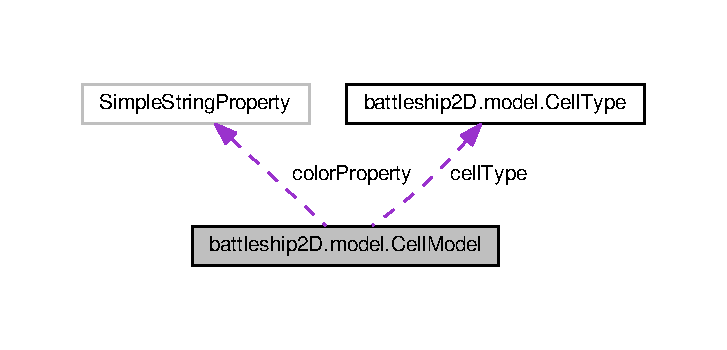
\includegraphics[width=349pt]{classbattleship2D_1_1model_1_1CellModel__coll__graph}
\end{center}
\end{figure}
\subsection*{Public Member Functions}
\begin{DoxyCompactItemize}
\item 
\hyperlink{classbattleship2D_1_1model_1_1CellModel_a9681f351cc619c88cb389c2f00a9a44d}{Cell\-Model} (\hyperlink{enumbattleship2D_1_1model_1_1CellType}{Cell\-Type} \hyperlink{classbattleship2D_1_1model_1_1CellModel_a5c1cadcce5c5639ae76d6d092fa8d510}{cell\-Type}, Integer \hyperlink{classbattleship2D_1_1model_1_1CellModel_a13643b1cd9553923ad542cf6c594d3c3}{id})
\begin{DoxyCompactList}\small\item\em Constructor. \end{DoxyCompactList}\item 
String \hyperlink{classbattleship2D_1_1model_1_1CellModel_aca1e2e88cbd929dc24aa7de4f15bd7a2}{display} ()
\begin{DoxyCompactList}\small\item\em Displays informations. \end{DoxyCompactList}\item 
\hyperlink{enumbattleship2D_1_1model_1_1CellType}{Cell\-Type} \hyperlink{classbattleship2D_1_1model_1_1CellModel_ae5c252d3bf4db6efc04f257096ff5522}{get\-Cell\-Type} ()
\item 
final void \hyperlink{classbattleship2D_1_1model_1_1CellModel_aa4b33ed17badf1b1058d554c23d324bc}{set\-Cell\-Type} (\hyperlink{enumbattleship2D_1_1model_1_1CellType}{Cell\-Type} \hyperlink{classbattleship2D_1_1model_1_1CellModel_a5c1cadcce5c5639ae76d6d092fa8d510}{cell\-Type})
\item 
Simple\-String\-Property \hyperlink{classbattleship2D_1_1model_1_1CellModel_ab76410b942fa598a6798da97256d0b23}{get\-Color\-Property} ()
\item 
Integer \hyperlink{classbattleship2D_1_1model_1_1CellModel_ac157a53ff0edf60519ce94795296da0d}{get\-Id} ()
\item 
final void \hyperlink{classbattleship2D_1_1model_1_1CellModel_ad3cf39763eb70d7ee5f4efa1553a5268}{set\-Id} (Integer \hyperlink{classbattleship2D_1_1model_1_1CellModel_a13643b1cd9553923ad542cf6c594d3c3}{id})
\end{DoxyCompactItemize}
\subsection*{Private Attributes}
\begin{DoxyCompactItemize}
\item 
\hyperlink{enumbattleship2D_1_1model_1_1CellType}{Cell\-Type} \hyperlink{classbattleship2D_1_1model_1_1CellModel_a5c1cadcce5c5639ae76d6d092fa8d510}{cell\-Type}
\begin{DoxyCompactList}\small\item\em Related type. \end{DoxyCompactList}\item 
final Simple\-String\-Property \hyperlink{classbattleship2D_1_1model_1_1CellModel_a35a8bdca8ab2e2a3a3d393f8707638fc}{color\-Property}
\begin{DoxyCompactList}\small\item\em Store the associated color. \end{DoxyCompactList}\item 
Integer \hyperlink{classbattleship2D_1_1model_1_1CellModel_a13643b1cd9553923ad542cf6c594d3c3}{id}
\begin{DoxyCompactList}\small\item\em Unique identifier. \end{DoxyCompactList}\end{DoxyCompactItemize}


\subsection{Detailed Description}
Board model element. 

\begin{DoxyAuthor}{Author}
xaviator 
\end{DoxyAuthor}


\subsection{Constructor \& Destructor Documentation}
\hypertarget{classbattleship2D_1_1model_1_1CellModel_a9681f351cc619c88cb389c2f00a9a44d}{\index{battleship2\-D\-::model\-::\-Cell\-Model@{battleship2\-D\-::model\-::\-Cell\-Model}!Cell\-Model@{Cell\-Model}}
\index{Cell\-Model@{Cell\-Model}!battleship2D::model::CellModel@{battleship2\-D\-::model\-::\-Cell\-Model}}
\subsubsection[{Cell\-Model}]{\setlength{\rightskip}{0pt plus 5cm}battleship2\-D.\-model.\-Cell\-Model.\-Cell\-Model (
\begin{DoxyParamCaption}
\item[{{\bf Cell\-Type}}]{cell\-Type, }
\item[{Integer}]{id}
\end{DoxyParamCaption}
)}}\label{classbattleship2D_1_1model_1_1CellModel_a9681f351cc619c88cb389c2f00a9a44d}


Constructor. 


\begin{DoxyParams}{Parameters}
{\em cell\-Type} & -\/ associated cell type \\
\hline
{\em id} & -\/ identifier \\
\hline
\end{DoxyParams}


\subsection{Member Function Documentation}
\hypertarget{classbattleship2D_1_1model_1_1CellModel_aca1e2e88cbd929dc24aa7de4f15bd7a2}{\index{battleship2\-D\-::model\-::\-Cell\-Model@{battleship2\-D\-::model\-::\-Cell\-Model}!display@{display}}
\index{display@{display}!battleship2D::model::CellModel@{battleship2\-D\-::model\-::\-Cell\-Model}}
\subsubsection[{display}]{\setlength{\rightskip}{0pt plus 5cm}String battleship2\-D.\-model.\-Cell\-Model.\-display (
\begin{DoxyParamCaption}
{}
\end{DoxyParamCaption}
)}}\label{classbattleship2D_1_1model_1_1CellModel_aca1e2e88cbd929dc24aa7de4f15bd7a2}


Displays informations. 

\begin{DoxyReturn}{Returns}
a brief description 
\end{DoxyReturn}
\hypertarget{classbattleship2D_1_1model_1_1CellModel_ae5c252d3bf4db6efc04f257096ff5522}{\index{battleship2\-D\-::model\-::\-Cell\-Model@{battleship2\-D\-::model\-::\-Cell\-Model}!get\-Cell\-Type@{get\-Cell\-Type}}
\index{get\-Cell\-Type@{get\-Cell\-Type}!battleship2D::model::CellModel@{battleship2\-D\-::model\-::\-Cell\-Model}}
\subsubsection[{get\-Cell\-Type}]{\setlength{\rightskip}{0pt plus 5cm}{\bf Cell\-Type} battleship2\-D.\-model.\-Cell\-Model.\-get\-Cell\-Type (
\begin{DoxyParamCaption}
{}
\end{DoxyParamCaption}
)}}\label{classbattleship2D_1_1model_1_1CellModel_ae5c252d3bf4db6efc04f257096ff5522}
\hypertarget{classbattleship2D_1_1model_1_1CellModel_ab76410b942fa598a6798da97256d0b23}{\index{battleship2\-D\-::model\-::\-Cell\-Model@{battleship2\-D\-::model\-::\-Cell\-Model}!get\-Color\-Property@{get\-Color\-Property}}
\index{get\-Color\-Property@{get\-Color\-Property}!battleship2D::model::CellModel@{battleship2\-D\-::model\-::\-Cell\-Model}}
\subsubsection[{get\-Color\-Property}]{\setlength{\rightskip}{0pt plus 5cm}Simple\-String\-Property battleship2\-D.\-model.\-Cell\-Model.\-get\-Color\-Property (
\begin{DoxyParamCaption}
{}
\end{DoxyParamCaption}
)}}\label{classbattleship2D_1_1model_1_1CellModel_ab76410b942fa598a6798da97256d0b23}
\hypertarget{classbattleship2D_1_1model_1_1CellModel_ac157a53ff0edf60519ce94795296da0d}{\index{battleship2\-D\-::model\-::\-Cell\-Model@{battleship2\-D\-::model\-::\-Cell\-Model}!get\-Id@{get\-Id}}
\index{get\-Id@{get\-Id}!battleship2D::model::CellModel@{battleship2\-D\-::model\-::\-Cell\-Model}}
\subsubsection[{get\-Id}]{\setlength{\rightskip}{0pt plus 5cm}Integer battleship2\-D.\-model.\-Cell\-Model.\-get\-Id (
\begin{DoxyParamCaption}
{}
\end{DoxyParamCaption}
)}}\label{classbattleship2D_1_1model_1_1CellModel_ac157a53ff0edf60519ce94795296da0d}
\hypertarget{classbattleship2D_1_1model_1_1CellModel_aa4b33ed17badf1b1058d554c23d324bc}{\index{battleship2\-D\-::model\-::\-Cell\-Model@{battleship2\-D\-::model\-::\-Cell\-Model}!set\-Cell\-Type@{set\-Cell\-Type}}
\index{set\-Cell\-Type@{set\-Cell\-Type}!battleship2D::model::CellModel@{battleship2\-D\-::model\-::\-Cell\-Model}}
\subsubsection[{set\-Cell\-Type}]{\setlength{\rightskip}{0pt plus 5cm}final void battleship2\-D.\-model.\-Cell\-Model.\-set\-Cell\-Type (
\begin{DoxyParamCaption}
\item[{{\bf Cell\-Type}}]{cell\-Type}
\end{DoxyParamCaption}
)}}\label{classbattleship2D_1_1model_1_1CellModel_aa4b33ed17badf1b1058d554c23d324bc}
\hypertarget{classbattleship2D_1_1model_1_1CellModel_ad3cf39763eb70d7ee5f4efa1553a5268}{\index{battleship2\-D\-::model\-::\-Cell\-Model@{battleship2\-D\-::model\-::\-Cell\-Model}!set\-Id@{set\-Id}}
\index{set\-Id@{set\-Id}!battleship2D::model::CellModel@{battleship2\-D\-::model\-::\-Cell\-Model}}
\subsubsection[{set\-Id}]{\setlength{\rightskip}{0pt plus 5cm}final void battleship2\-D.\-model.\-Cell\-Model.\-set\-Id (
\begin{DoxyParamCaption}
\item[{Integer}]{id}
\end{DoxyParamCaption}
)}}\label{classbattleship2D_1_1model_1_1CellModel_ad3cf39763eb70d7ee5f4efa1553a5268}


\subsection{Member Data Documentation}
\hypertarget{classbattleship2D_1_1model_1_1CellModel_a5c1cadcce5c5639ae76d6d092fa8d510}{\index{battleship2\-D\-::model\-::\-Cell\-Model@{battleship2\-D\-::model\-::\-Cell\-Model}!cell\-Type@{cell\-Type}}
\index{cell\-Type@{cell\-Type}!battleship2D::model::CellModel@{battleship2\-D\-::model\-::\-Cell\-Model}}
\subsubsection[{cell\-Type}]{\setlength{\rightskip}{0pt plus 5cm}{\bf Cell\-Type} battleship2\-D.\-model.\-Cell\-Model.\-cell\-Type\hspace{0.3cm}{\ttfamily [private]}}}\label{classbattleship2D_1_1model_1_1CellModel_a5c1cadcce5c5639ae76d6d092fa8d510}


Related type. 

\hypertarget{classbattleship2D_1_1model_1_1CellModel_a35a8bdca8ab2e2a3a3d393f8707638fc}{\index{battleship2\-D\-::model\-::\-Cell\-Model@{battleship2\-D\-::model\-::\-Cell\-Model}!color\-Property@{color\-Property}}
\index{color\-Property@{color\-Property}!battleship2D::model::CellModel@{battleship2\-D\-::model\-::\-Cell\-Model}}
\subsubsection[{color\-Property}]{\setlength{\rightskip}{0pt plus 5cm}final Simple\-String\-Property battleship2\-D.\-model.\-Cell\-Model.\-color\-Property\hspace{0.3cm}{\ttfamily [private]}}}\label{classbattleship2D_1_1model_1_1CellModel_a35a8bdca8ab2e2a3a3d393f8707638fc}


Store the associated color. 

\hypertarget{classbattleship2D_1_1model_1_1CellModel_a13643b1cd9553923ad542cf6c594d3c3}{\index{battleship2\-D\-::model\-::\-Cell\-Model@{battleship2\-D\-::model\-::\-Cell\-Model}!id@{id}}
\index{id@{id}!battleship2D::model::CellModel@{battleship2\-D\-::model\-::\-Cell\-Model}}
\subsubsection[{id}]{\setlength{\rightskip}{0pt plus 5cm}Integer battleship2\-D.\-model.\-Cell\-Model.\-id\hspace{0.3cm}{\ttfamily [private]}}}\label{classbattleship2D_1_1model_1_1CellModel_a13643b1cd9553923ad542cf6c594d3c3}


Unique identifier. 



The documentation for this class was generated from the following file\-:\begin{DoxyCompactItemize}
\item 
/home/xaviator/\-Enseignements/2015-\/2016/\-S\-F\-A/\-M1-\/\-Info/\-I\-H\-M/\-Battle\-Ship2\-D\-\_\-students/battleship2\-D/model/\hyperlink{CellModel_8java}{Cell\-Model.\-java}\end{DoxyCompactItemize}

\hypertarget{enumbattleship2D_1_1model_1_1CellType}{\section{battleship2\-D.\-model.\-Cell\-Type Enum Reference}
\label{enumbattleship2D_1_1model_1_1CellType}\index{battleship2\-D.\-model.\-Cell\-Type@{battleship2\-D.\-model.\-Cell\-Type}}
}


Cell Types.  


\subsection*{Public Member Functions}
\begin{DoxyCompactItemize}
\item 
boolean \hyperlink{enumbattleship2D_1_1model_1_1CellType_a704b9068d644f547792823905a772f2a}{is\-A\-Ship} ()
\begin{DoxyCompactList}\small\item\em Check whether this \hyperlink{enumbattleship2D_1_1model_1_1CellType}{Cell\-Type} is a ship. \end{DoxyCompactList}\item 
String \hyperlink{enumbattleship2D_1_1model_1_1CellType_aed7191d88c4d7712a6ca555c1a715243}{get\-Description} ()
\item 
String \hyperlink{enumbattleship2D_1_1model_1_1CellType_a2af2beb0ae9a067bba1c6ddea4f9d0ae}{get\-Appearance} ()
\end{DoxyCompactItemize}
\subsection*{Static Public Member Functions}
\begin{DoxyCompactItemize}
\item 
static \hyperlink{enumbattleship2D_1_1model_1_1ShipType}{Ship\-Type} \hyperlink{enumbattleship2D_1_1model_1_1CellType_a41eeb4c56d05d406a34cc4ad9996c329}{cell\-Type\-To\-Ship\-Type} (\hyperlink{enumbattleship2D_1_1model_1_1CellType}{Cell\-Type} cell\-Type)
\begin{DoxyCompactList}\small\item\em Converts a \hyperlink{enumbattleship2D_1_1model_1_1CellType}{Cell\-Type} into a \hyperlink{enumbattleship2D_1_1model_1_1ShipType}{Ship\-Type}. \end{DoxyCompactList}\item 
static \hyperlink{enumbattleship2D_1_1model_1_1CellType}{Cell\-Type} \hyperlink{enumbattleship2D_1_1model_1_1CellType_a5d3b8fd30d9afa7a8505074b87850719}{ship\-Type\-To\-Cell\-Type} (\hyperlink{enumbattleship2D_1_1model_1_1ShipType}{Ship\-Type} ship\-Type)
\begin{DoxyCompactList}\small\item\em Converts a \hyperlink{enumbattleship2D_1_1model_1_1ShipType}{Ship\-Type} into a \hyperlink{enumbattleship2D_1_1model_1_1CellType}{Cell\-Type}. \end{DoxyCompactList}\end{DoxyCompactItemize}
\subsection*{Public Attributes}
\begin{DoxyCompactItemize}
\item 
\hyperlink{enumbattleship2D_1_1model_1_1CellType_a50f3594d7ffcf1d25b3ff7ba63559d7b}{A\-V\-A\-I\-L\-A\-B\-L\-E\-\_\-\-L\-O\-C\-A\-T\-I\-O\-N} =(\char`\"{}Available\char`\"{}, \char`\"{}-\/fx-\/background-\/color\-: aquamarine\char`\"{})
\item 
\hyperlink{enumbattleship2D_1_1model_1_1CellType_af1cb88f225ce4a6bb31ecc9c44b1ba43}{B\-A\-T\-T\-L\-E\-S\-H\-I\-P} =(Ship\-Type.\-B\-A\-T\-T\-L\-E\-S\-H\-I\-P)
\item 
\hyperlink{enumbattleship2D_1_1model_1_1CellType_a3c23cb8e58884afac9826793bdca060d}{C\-A\-R\-R\-I\-E\-R} =(Ship\-Type.\-C\-A\-R\-R\-I\-E\-R)
\item 
\hyperlink{enumbattleship2D_1_1model_1_1CellType_a45ec63311bbed0763d44b0e6428da6f4}{C\-R\-U\-I\-S\-E\-R} =(Ship\-Type.\-C\-R\-U\-I\-S\-E\-R)
\item 
\hyperlink{enumbattleship2D_1_1model_1_1CellType_a89b7d59bf01fbd390393926de5b840b6}{D\-E\-S\-T\-R\-O\-Y\-E\-R} =(Ship\-Type.\-D\-E\-S\-T\-R\-O\-Y\-E\-R)
\item 
\hyperlink{enumbattleship2D_1_1model_1_1CellType_aedac6244a22b1b1a7a7dc2887ea3827a}{H\-I\-T} =(\char`\"{}Hit\char`\"{}, \char`\"{}-\/fx-\/background-\/image\-: url(\textbackslash{}\char`\"{}battleship2\-D/pictures/ship-\/explosion.\-jpg\textbackslash{}\char`\"{})\char`\"{})
\item 
\hyperlink{enumbattleship2D_1_1model_1_1CellType_af010e793915bcca6ccc54b59d6687b0f}{O\-C\-E\-A\-N} =(\char`\"{}Ocean\char`\"{}, \char`\"{}-\/fx-\/background-\/image\-: url(\textbackslash{}\char`\"{}battleship2\-D/pictures/ocean.\-jpeg\textbackslash{}\char`\"{})\char`\"{})
\item 
\hyperlink{enumbattleship2D_1_1model_1_1CellType_af0cd87a32526f247a9347043d4c57a6e}{S\-U\-B\-M\-A\-R\-I\-N\-E} =(Ship\-Type.\-S\-U\-B\-M\-A\-R\-I\-N\-E)
\item 
\hyperlink{enumbattleship2D_1_1model_1_1CellType_a8d4deb923c1df4cd4148f298e4adfdfb}{U\-N\-K\-N\-O\-W\-N} =(\char`\"{}Unknown\char`\"{}, \char`\"{}-\/fx-\/background-\/color\-: black\char`\"{})
\end{DoxyCompactItemize}
\subsection*{Private Member Functions}
\begin{DoxyCompactItemize}
\item 
\hyperlink{enumbattleship2D_1_1model_1_1CellType_aea27835e7561cfecd0aedb835390d5fb}{Cell\-Type} (final String \hyperlink{enumbattleship2D_1_1model_1_1CellType_a523e78aea9b3eb082fcbe1af6f7580d2}{description}, final String \hyperlink{enumbattleship2D_1_1model_1_1CellType_a164d67bf5b6b674e63a766b9897ec3f4}{appearance})
\begin{DoxyCompactList}\small\item\em Constructor. \end{DoxyCompactList}\item 
\hyperlink{enumbattleship2D_1_1model_1_1CellType_a113ce6d9cd8bb4bae16752c42f9e521f}{Cell\-Type} (\hyperlink{enumbattleship2D_1_1model_1_1ShipType}{Ship\-Type} ship\-Type)
\begin{DoxyCompactList}\small\item\em Constructor. \end{DoxyCompactList}\end{DoxyCompactItemize}
\subsection*{Private Attributes}
\begin{DoxyCompactItemize}
\item 
final String \hyperlink{enumbattleship2D_1_1model_1_1CellType_a164d67bf5b6b674e63a766b9897ec3f4}{appearance}
\begin{DoxyCompactList}\small\item\em Rendering either as a color or an image. \end{DoxyCompactList}\item 
final String \hyperlink{enumbattleship2D_1_1model_1_1CellType_a523e78aea9b3eb082fcbe1af6f7580d2}{description}
\begin{DoxyCompactList}\small\item\em Short description. \end{DoxyCompactList}\end{DoxyCompactItemize}


\subsection{Detailed Description}
Cell Types. 

\begin{DoxyAuthor}{Author}
xaviator 
\end{DoxyAuthor}


\subsection{Constructor \& Destructor Documentation}
\hypertarget{enumbattleship2D_1_1model_1_1CellType_aea27835e7561cfecd0aedb835390d5fb}{\index{battleship2\-D\-::model\-::\-Cell\-Type@{battleship2\-D\-::model\-::\-Cell\-Type}!Cell\-Type@{Cell\-Type}}
\index{Cell\-Type@{Cell\-Type}!battleship2D::model::CellType@{battleship2\-D\-::model\-::\-Cell\-Type}}
\subsubsection[{Cell\-Type}]{\setlength{\rightskip}{0pt plus 5cm}battleship2\-D.\-model.\-Cell\-Type.\-Cell\-Type (
\begin{DoxyParamCaption}
\item[{final String}]{description, }
\item[{final String}]{appearance}
\end{DoxyParamCaption}
)\hspace{0.3cm}{\ttfamily [private]}}}\label{enumbattleship2D_1_1model_1_1CellType_aea27835e7561cfecd0aedb835390d5fb}


Constructor. 


\begin{DoxyParams}{Parameters}
{\em description} & -\/ short description \\
\hline
{\em appearance} & -\/ related appearance \\
\hline
\end{DoxyParams}
\hypertarget{enumbattleship2D_1_1model_1_1CellType_a113ce6d9cd8bb4bae16752c42f9e521f}{\index{battleship2\-D\-::model\-::\-Cell\-Type@{battleship2\-D\-::model\-::\-Cell\-Type}!Cell\-Type@{Cell\-Type}}
\index{Cell\-Type@{Cell\-Type}!battleship2D::model::CellType@{battleship2\-D\-::model\-::\-Cell\-Type}}
\subsubsection[{Cell\-Type}]{\setlength{\rightskip}{0pt plus 5cm}battleship2\-D.\-model.\-Cell\-Type.\-Cell\-Type (
\begin{DoxyParamCaption}
\item[{{\bf Ship\-Type}}]{ship\-Type}
\end{DoxyParamCaption}
)\hspace{0.3cm}{\ttfamily [private]}}}\label{enumbattleship2D_1_1model_1_1CellType_a113ce6d9cd8bb4bae16752c42f9e521f}


Constructor. 


\begin{DoxyParams}{Parameters}
{\em description} & -\/ short description \\
\hline
{\em appearance} & -\/ related appearance \\
\hline
\end{DoxyParams}


\subsection{Member Function Documentation}
\hypertarget{enumbattleship2D_1_1model_1_1CellType_a41eeb4c56d05d406a34cc4ad9996c329}{\index{battleship2\-D\-::model\-::\-Cell\-Type@{battleship2\-D\-::model\-::\-Cell\-Type}!cell\-Type\-To\-Ship\-Type@{cell\-Type\-To\-Ship\-Type}}
\index{cell\-Type\-To\-Ship\-Type@{cell\-Type\-To\-Ship\-Type}!battleship2D::model::CellType@{battleship2\-D\-::model\-::\-Cell\-Type}}
\subsubsection[{cell\-Type\-To\-Ship\-Type}]{\setlength{\rightskip}{0pt plus 5cm}static {\bf Ship\-Type} battleship2\-D.\-model.\-Cell\-Type.\-cell\-Type\-To\-Ship\-Type (
\begin{DoxyParamCaption}
\item[{{\bf Cell\-Type}}]{cell\-Type}
\end{DoxyParamCaption}
)\hspace{0.3cm}{\ttfamily [static]}}}\label{enumbattleship2D_1_1model_1_1CellType_a41eeb4c56d05d406a34cc4ad9996c329}


Converts a \hyperlink{enumbattleship2D_1_1model_1_1CellType}{Cell\-Type} into a \hyperlink{enumbattleship2D_1_1model_1_1ShipType}{Ship\-Type}. 


\begin{DoxyParams}{Parameters}
{\em cell\-Type} & -\/ cell type to deal with \\
\hline
\end{DoxyParams}
\begin{DoxyReturn}{Returns}
the matching ship type 
\end{DoxyReturn}
\hypertarget{enumbattleship2D_1_1model_1_1CellType_a2af2beb0ae9a067bba1c6ddea4f9d0ae}{\index{battleship2\-D\-::model\-::\-Cell\-Type@{battleship2\-D\-::model\-::\-Cell\-Type}!get\-Appearance@{get\-Appearance}}
\index{get\-Appearance@{get\-Appearance}!battleship2D::model::CellType@{battleship2\-D\-::model\-::\-Cell\-Type}}
\subsubsection[{get\-Appearance}]{\setlength{\rightskip}{0pt plus 5cm}String battleship2\-D.\-model.\-Cell\-Type.\-get\-Appearance (
\begin{DoxyParamCaption}
{}
\end{DoxyParamCaption}
)}}\label{enumbattleship2D_1_1model_1_1CellType_a2af2beb0ae9a067bba1c6ddea4f9d0ae}
\hypertarget{enumbattleship2D_1_1model_1_1CellType_aed7191d88c4d7712a6ca555c1a715243}{\index{battleship2\-D\-::model\-::\-Cell\-Type@{battleship2\-D\-::model\-::\-Cell\-Type}!get\-Description@{get\-Description}}
\index{get\-Description@{get\-Description}!battleship2D::model::CellType@{battleship2\-D\-::model\-::\-Cell\-Type}}
\subsubsection[{get\-Description}]{\setlength{\rightskip}{0pt plus 5cm}String battleship2\-D.\-model.\-Cell\-Type.\-get\-Description (
\begin{DoxyParamCaption}
{}
\end{DoxyParamCaption}
)}}\label{enumbattleship2D_1_1model_1_1CellType_aed7191d88c4d7712a6ca555c1a715243}
\hypertarget{enumbattleship2D_1_1model_1_1CellType_a704b9068d644f547792823905a772f2a}{\index{battleship2\-D\-::model\-::\-Cell\-Type@{battleship2\-D\-::model\-::\-Cell\-Type}!is\-A\-Ship@{is\-A\-Ship}}
\index{is\-A\-Ship@{is\-A\-Ship}!battleship2D::model::CellType@{battleship2\-D\-::model\-::\-Cell\-Type}}
\subsubsection[{is\-A\-Ship}]{\setlength{\rightskip}{0pt plus 5cm}boolean battleship2\-D.\-model.\-Cell\-Type.\-is\-A\-Ship (
\begin{DoxyParamCaption}
{}
\end{DoxyParamCaption}
)}}\label{enumbattleship2D_1_1model_1_1CellType_a704b9068d644f547792823905a772f2a}


Check whether this \hyperlink{enumbattleship2D_1_1model_1_1CellType}{Cell\-Type} is a ship. 

\begin{DoxyReturn}{Returns}
true if this is a ship, false otherwise 
\end{DoxyReturn}
\hypertarget{enumbattleship2D_1_1model_1_1CellType_a5d3b8fd30d9afa7a8505074b87850719}{\index{battleship2\-D\-::model\-::\-Cell\-Type@{battleship2\-D\-::model\-::\-Cell\-Type}!ship\-Type\-To\-Cell\-Type@{ship\-Type\-To\-Cell\-Type}}
\index{ship\-Type\-To\-Cell\-Type@{ship\-Type\-To\-Cell\-Type}!battleship2D::model::CellType@{battleship2\-D\-::model\-::\-Cell\-Type}}
\subsubsection[{ship\-Type\-To\-Cell\-Type}]{\setlength{\rightskip}{0pt plus 5cm}static {\bf Cell\-Type} battleship2\-D.\-model.\-Cell\-Type.\-ship\-Type\-To\-Cell\-Type (
\begin{DoxyParamCaption}
\item[{{\bf Ship\-Type}}]{ship\-Type}
\end{DoxyParamCaption}
)\hspace{0.3cm}{\ttfamily [static]}}}\label{enumbattleship2D_1_1model_1_1CellType_a5d3b8fd30d9afa7a8505074b87850719}


Converts a \hyperlink{enumbattleship2D_1_1model_1_1ShipType}{Ship\-Type} into a \hyperlink{enumbattleship2D_1_1model_1_1CellType}{Cell\-Type}. 


\begin{DoxyParams}{Parameters}
{\em ship\-Type} & -\/ the ship type to convert \\
\hline
\end{DoxyParams}
\begin{DoxyReturn}{Returns}
the matching cell type 
\end{DoxyReturn}


\subsection{Member Data Documentation}
\hypertarget{enumbattleship2D_1_1model_1_1CellType_a164d67bf5b6b674e63a766b9897ec3f4}{\index{battleship2\-D\-::model\-::\-Cell\-Type@{battleship2\-D\-::model\-::\-Cell\-Type}!appearance@{appearance}}
\index{appearance@{appearance}!battleship2D::model::CellType@{battleship2\-D\-::model\-::\-Cell\-Type}}
\subsubsection[{appearance}]{\setlength{\rightskip}{0pt plus 5cm}final String battleship2\-D.\-model.\-Cell\-Type.\-appearance\hspace{0.3cm}{\ttfamily [private]}}}\label{enumbattleship2D_1_1model_1_1CellType_a164d67bf5b6b674e63a766b9897ec3f4}


Rendering either as a color or an image. 

\hypertarget{enumbattleship2D_1_1model_1_1CellType_a50f3594d7ffcf1d25b3ff7ba63559d7b}{\index{battleship2\-D\-::model\-::\-Cell\-Type@{battleship2\-D\-::model\-::\-Cell\-Type}!A\-V\-A\-I\-L\-A\-B\-L\-E\-\_\-\-L\-O\-C\-A\-T\-I\-O\-N@{A\-V\-A\-I\-L\-A\-B\-L\-E\-\_\-\-L\-O\-C\-A\-T\-I\-O\-N}}
\index{A\-V\-A\-I\-L\-A\-B\-L\-E\-\_\-\-L\-O\-C\-A\-T\-I\-O\-N@{A\-V\-A\-I\-L\-A\-B\-L\-E\-\_\-\-L\-O\-C\-A\-T\-I\-O\-N}!battleship2D::model::CellType@{battleship2\-D\-::model\-::\-Cell\-Type}}
\subsubsection[{A\-V\-A\-I\-L\-A\-B\-L\-E\-\_\-\-L\-O\-C\-A\-T\-I\-O\-N}]{\setlength{\rightskip}{0pt plus 5cm}battleship2\-D.\-model.\-Cell\-Type.\-A\-V\-A\-I\-L\-A\-B\-L\-E\-\_\-\-L\-O\-C\-A\-T\-I\-O\-N =(\char`\"{}Available\char`\"{}, \char`\"{}-\/fx-\/background-\/color\-: aquamarine\char`\"{})}}\label{enumbattleship2D_1_1model_1_1CellType_a50f3594d7ffcf1d25b3ff7ba63559d7b}
\hypertarget{enumbattleship2D_1_1model_1_1CellType_af1cb88f225ce4a6bb31ecc9c44b1ba43}{\index{battleship2\-D\-::model\-::\-Cell\-Type@{battleship2\-D\-::model\-::\-Cell\-Type}!B\-A\-T\-T\-L\-E\-S\-H\-I\-P@{B\-A\-T\-T\-L\-E\-S\-H\-I\-P}}
\index{B\-A\-T\-T\-L\-E\-S\-H\-I\-P@{B\-A\-T\-T\-L\-E\-S\-H\-I\-P}!battleship2D::model::CellType@{battleship2\-D\-::model\-::\-Cell\-Type}}
\subsubsection[{B\-A\-T\-T\-L\-E\-S\-H\-I\-P}]{\setlength{\rightskip}{0pt plus 5cm}battleship2\-D.\-model.\-Cell\-Type.\-B\-A\-T\-T\-L\-E\-S\-H\-I\-P =(Ship\-Type.\-B\-A\-T\-T\-L\-E\-S\-H\-I\-P)}}\label{enumbattleship2D_1_1model_1_1CellType_af1cb88f225ce4a6bb31ecc9c44b1ba43}
\hypertarget{enumbattleship2D_1_1model_1_1CellType_a3c23cb8e58884afac9826793bdca060d}{\index{battleship2\-D\-::model\-::\-Cell\-Type@{battleship2\-D\-::model\-::\-Cell\-Type}!C\-A\-R\-R\-I\-E\-R@{C\-A\-R\-R\-I\-E\-R}}
\index{C\-A\-R\-R\-I\-E\-R@{C\-A\-R\-R\-I\-E\-R}!battleship2D::model::CellType@{battleship2\-D\-::model\-::\-Cell\-Type}}
\subsubsection[{C\-A\-R\-R\-I\-E\-R}]{\setlength{\rightskip}{0pt plus 5cm}battleship2\-D.\-model.\-Cell\-Type.\-C\-A\-R\-R\-I\-E\-R =(Ship\-Type.\-C\-A\-R\-R\-I\-E\-R)}}\label{enumbattleship2D_1_1model_1_1CellType_a3c23cb8e58884afac9826793bdca060d}
\hypertarget{enumbattleship2D_1_1model_1_1CellType_a45ec63311bbed0763d44b0e6428da6f4}{\index{battleship2\-D\-::model\-::\-Cell\-Type@{battleship2\-D\-::model\-::\-Cell\-Type}!C\-R\-U\-I\-S\-E\-R@{C\-R\-U\-I\-S\-E\-R}}
\index{C\-R\-U\-I\-S\-E\-R@{C\-R\-U\-I\-S\-E\-R}!battleship2D::model::CellType@{battleship2\-D\-::model\-::\-Cell\-Type}}
\subsubsection[{C\-R\-U\-I\-S\-E\-R}]{\setlength{\rightskip}{0pt plus 5cm}battleship2\-D.\-model.\-Cell\-Type.\-C\-R\-U\-I\-S\-E\-R =(Ship\-Type.\-C\-R\-U\-I\-S\-E\-R)}}\label{enumbattleship2D_1_1model_1_1CellType_a45ec63311bbed0763d44b0e6428da6f4}
\hypertarget{enumbattleship2D_1_1model_1_1CellType_a523e78aea9b3eb082fcbe1af6f7580d2}{\index{battleship2\-D\-::model\-::\-Cell\-Type@{battleship2\-D\-::model\-::\-Cell\-Type}!description@{description}}
\index{description@{description}!battleship2D::model::CellType@{battleship2\-D\-::model\-::\-Cell\-Type}}
\subsubsection[{description}]{\setlength{\rightskip}{0pt plus 5cm}final String battleship2\-D.\-model.\-Cell\-Type.\-description\hspace{0.3cm}{\ttfamily [private]}}}\label{enumbattleship2D_1_1model_1_1CellType_a523e78aea9b3eb082fcbe1af6f7580d2}


Short description. 

\hypertarget{enumbattleship2D_1_1model_1_1CellType_a89b7d59bf01fbd390393926de5b840b6}{\index{battleship2\-D\-::model\-::\-Cell\-Type@{battleship2\-D\-::model\-::\-Cell\-Type}!D\-E\-S\-T\-R\-O\-Y\-E\-R@{D\-E\-S\-T\-R\-O\-Y\-E\-R}}
\index{D\-E\-S\-T\-R\-O\-Y\-E\-R@{D\-E\-S\-T\-R\-O\-Y\-E\-R}!battleship2D::model::CellType@{battleship2\-D\-::model\-::\-Cell\-Type}}
\subsubsection[{D\-E\-S\-T\-R\-O\-Y\-E\-R}]{\setlength{\rightskip}{0pt plus 5cm}battleship2\-D.\-model.\-Cell\-Type.\-D\-E\-S\-T\-R\-O\-Y\-E\-R =(Ship\-Type.\-D\-E\-S\-T\-R\-O\-Y\-E\-R)}}\label{enumbattleship2D_1_1model_1_1CellType_a89b7d59bf01fbd390393926de5b840b6}
\hypertarget{enumbattleship2D_1_1model_1_1CellType_aedac6244a22b1b1a7a7dc2887ea3827a}{\index{battleship2\-D\-::model\-::\-Cell\-Type@{battleship2\-D\-::model\-::\-Cell\-Type}!H\-I\-T@{H\-I\-T}}
\index{H\-I\-T@{H\-I\-T}!battleship2D::model::CellType@{battleship2\-D\-::model\-::\-Cell\-Type}}
\subsubsection[{H\-I\-T}]{\setlength{\rightskip}{0pt plus 5cm}battleship2\-D.\-model.\-Cell\-Type.\-H\-I\-T =(\char`\"{}Hit\char`\"{}, \char`\"{}-\/fx-\/background-\/image\-: url(\textbackslash{}\char`\"{}battleship2\-D/pictures/ship-\/explosion.\-jpg\textbackslash{}\char`\"{})\char`\"{})}}\label{enumbattleship2D_1_1model_1_1CellType_aedac6244a22b1b1a7a7dc2887ea3827a}
\hypertarget{enumbattleship2D_1_1model_1_1CellType_af010e793915bcca6ccc54b59d6687b0f}{\index{battleship2\-D\-::model\-::\-Cell\-Type@{battleship2\-D\-::model\-::\-Cell\-Type}!O\-C\-E\-A\-N@{O\-C\-E\-A\-N}}
\index{O\-C\-E\-A\-N@{O\-C\-E\-A\-N}!battleship2D::model::CellType@{battleship2\-D\-::model\-::\-Cell\-Type}}
\subsubsection[{O\-C\-E\-A\-N}]{\setlength{\rightskip}{0pt plus 5cm}battleship2\-D.\-model.\-Cell\-Type.\-O\-C\-E\-A\-N =(\char`\"{}Ocean\char`\"{}, \char`\"{}-\/fx-\/background-\/image\-: url(\textbackslash{}\char`\"{}battleship2\-D/pictures/ocean.\-jpeg\textbackslash{}\char`\"{})\char`\"{})}}\label{enumbattleship2D_1_1model_1_1CellType_af010e793915bcca6ccc54b59d6687b0f}
\hypertarget{enumbattleship2D_1_1model_1_1CellType_af0cd87a32526f247a9347043d4c57a6e}{\index{battleship2\-D\-::model\-::\-Cell\-Type@{battleship2\-D\-::model\-::\-Cell\-Type}!S\-U\-B\-M\-A\-R\-I\-N\-E@{S\-U\-B\-M\-A\-R\-I\-N\-E}}
\index{S\-U\-B\-M\-A\-R\-I\-N\-E@{S\-U\-B\-M\-A\-R\-I\-N\-E}!battleship2D::model::CellType@{battleship2\-D\-::model\-::\-Cell\-Type}}
\subsubsection[{S\-U\-B\-M\-A\-R\-I\-N\-E}]{\setlength{\rightskip}{0pt plus 5cm}battleship2\-D.\-model.\-Cell\-Type.\-S\-U\-B\-M\-A\-R\-I\-N\-E =(Ship\-Type.\-S\-U\-B\-M\-A\-R\-I\-N\-E)}}\label{enumbattleship2D_1_1model_1_1CellType_af0cd87a32526f247a9347043d4c57a6e}
\hypertarget{enumbattleship2D_1_1model_1_1CellType_a8d4deb923c1df4cd4148f298e4adfdfb}{\index{battleship2\-D\-::model\-::\-Cell\-Type@{battleship2\-D\-::model\-::\-Cell\-Type}!U\-N\-K\-N\-O\-W\-N@{U\-N\-K\-N\-O\-W\-N}}
\index{U\-N\-K\-N\-O\-W\-N@{U\-N\-K\-N\-O\-W\-N}!battleship2D::model::CellType@{battleship2\-D\-::model\-::\-Cell\-Type}}
\subsubsection[{U\-N\-K\-N\-O\-W\-N}]{\setlength{\rightskip}{0pt plus 5cm}battleship2\-D.\-model.\-Cell\-Type.\-U\-N\-K\-N\-O\-W\-N =(\char`\"{}Unknown\char`\"{}, \char`\"{}-\/fx-\/background-\/color\-: black\char`\"{})}}\label{enumbattleship2D_1_1model_1_1CellType_a8d4deb923c1df4cd4148f298e4adfdfb}


The documentation for this enum was generated from the following file\-:\begin{DoxyCompactItemize}
\item 
/home/xaviator/\-Enseignements/2015-\/2016/\-S\-F\-A/\-M1-\/\-Info/\-I\-H\-M/\-Battle\-Ship2\-D\-\_\-students/battleship2\-D/model/\hyperlink{CellType_8java}{Cell\-Type.\-java}\end{DoxyCompactItemize}

\hypertarget{classbattleship2D_1_1model_1_1Coord2D}{\section{battleship2\-D.\-model.\-Coord2\-D Class Reference}
\label{classbattleship2D_1_1model_1_1Coord2D}\index{battleship2\-D.\-model.\-Coord2\-D@{battleship2\-D.\-model.\-Coord2\-D}}
}


(row,column) -\/ coordinates pair inside a 2\-D array  


\subsection*{Public Member Functions}
\begin{DoxyCompactItemize}
\item 
\hyperlink{classbattleship2D_1_1model_1_1Coord2D_ae46741217f55556ecb5d04d63eef7f71}{Coord2\-D} (int \hyperlink{classbattleship2D_1_1model_1_1Coord2D_a6f65494fedcc38fc14183bd1b84869a1}{row}, int \hyperlink{classbattleship2D_1_1model_1_1Coord2D_ab75c922fc86f340e5722297fa25a3bd8}{column})
\begin{DoxyCompactList}\small\item\em Constructor. \end{DoxyCompactList}\item 
int \hyperlink{classbattleship2D_1_1model_1_1Coord2D_a691c1fc2511b9c6bc888a8e17c8cc62e}{get\-Row} ()
\item 
final void \hyperlink{classbattleship2D_1_1model_1_1Coord2D_a0be3424c423bd438cdcceae7b829353c}{set\-Row} (int \hyperlink{classbattleship2D_1_1model_1_1Coord2D_a6f65494fedcc38fc14183bd1b84869a1}{row})
\item 
int \hyperlink{classbattleship2D_1_1model_1_1Coord2D_a36cde8143f4ba0dda88b5fbbb56076ff}{get\-Column} ()
\item 
final void \hyperlink{classbattleship2D_1_1model_1_1Coord2D_a9152c6f9e7d7600483d4b36c89acefce}{set\-Column} (int \hyperlink{classbattleship2D_1_1model_1_1Coord2D_ab75c922fc86f340e5722297fa25a3bd8}{column})
\end{DoxyCompactItemize}
\subsection*{Package Attributes}
\begin{DoxyCompactItemize}
\item 
int \hyperlink{classbattleship2D_1_1model_1_1Coord2D_a6f65494fedcc38fc14183bd1b84869a1}{row}
\end{DoxyCompactItemize}
\subsection*{Private Attributes}
\begin{DoxyCompactItemize}
\item 
int \hyperlink{classbattleship2D_1_1model_1_1Coord2D_ab75c922fc86f340e5722297fa25a3bd8}{column}
\begin{DoxyCompactList}\small\item\em 2\-D coordinates \end{DoxyCompactList}\end{DoxyCompactItemize}


\subsection{Detailed Description}
(row,column) -\/ coordinates pair inside a 2\-D array 

\begin{DoxyAuthor}{Author}
xaviator 
\end{DoxyAuthor}


\subsection{Constructor \& Destructor Documentation}
\hypertarget{classbattleship2D_1_1model_1_1Coord2D_ae46741217f55556ecb5d04d63eef7f71}{\index{battleship2\-D\-::model\-::\-Coord2\-D@{battleship2\-D\-::model\-::\-Coord2\-D}!Coord2\-D@{Coord2\-D}}
\index{Coord2\-D@{Coord2\-D}!battleship2D::model::Coord2D@{battleship2\-D\-::model\-::\-Coord2\-D}}
\subsubsection[{Coord2\-D}]{\setlength{\rightskip}{0pt plus 5cm}battleship2\-D.\-model.\-Coord2\-D.\-Coord2\-D (
\begin{DoxyParamCaption}
\item[{int}]{row, }
\item[{int}]{column}
\end{DoxyParamCaption}
)}}\label{classbattleship2D_1_1model_1_1Coord2D_ae46741217f55556ecb5d04d63eef7f71}


Constructor. 


\begin{DoxyParams}{Parameters}
{\em row} & -\/ new row value \\
\hline
{\em column} & new column value \\
\hline
\end{DoxyParams}


\subsection{Member Function Documentation}
\hypertarget{classbattleship2D_1_1model_1_1Coord2D_a36cde8143f4ba0dda88b5fbbb56076ff}{\index{battleship2\-D\-::model\-::\-Coord2\-D@{battleship2\-D\-::model\-::\-Coord2\-D}!get\-Column@{get\-Column}}
\index{get\-Column@{get\-Column}!battleship2D::model::Coord2D@{battleship2\-D\-::model\-::\-Coord2\-D}}
\subsubsection[{get\-Column}]{\setlength{\rightskip}{0pt plus 5cm}int battleship2\-D.\-model.\-Coord2\-D.\-get\-Column (
\begin{DoxyParamCaption}
{}
\end{DoxyParamCaption}
)}}\label{classbattleship2D_1_1model_1_1Coord2D_a36cde8143f4ba0dda88b5fbbb56076ff}
\hypertarget{classbattleship2D_1_1model_1_1Coord2D_a691c1fc2511b9c6bc888a8e17c8cc62e}{\index{battleship2\-D\-::model\-::\-Coord2\-D@{battleship2\-D\-::model\-::\-Coord2\-D}!get\-Row@{get\-Row}}
\index{get\-Row@{get\-Row}!battleship2D::model::Coord2D@{battleship2\-D\-::model\-::\-Coord2\-D}}
\subsubsection[{get\-Row}]{\setlength{\rightskip}{0pt plus 5cm}int battleship2\-D.\-model.\-Coord2\-D.\-get\-Row (
\begin{DoxyParamCaption}
{}
\end{DoxyParamCaption}
)}}\label{classbattleship2D_1_1model_1_1Coord2D_a691c1fc2511b9c6bc888a8e17c8cc62e}
\hypertarget{classbattleship2D_1_1model_1_1Coord2D_a9152c6f9e7d7600483d4b36c89acefce}{\index{battleship2\-D\-::model\-::\-Coord2\-D@{battleship2\-D\-::model\-::\-Coord2\-D}!set\-Column@{set\-Column}}
\index{set\-Column@{set\-Column}!battleship2D::model::Coord2D@{battleship2\-D\-::model\-::\-Coord2\-D}}
\subsubsection[{set\-Column}]{\setlength{\rightskip}{0pt plus 5cm}final void battleship2\-D.\-model.\-Coord2\-D.\-set\-Column (
\begin{DoxyParamCaption}
\item[{int}]{column}
\end{DoxyParamCaption}
)}}\label{classbattleship2D_1_1model_1_1Coord2D_a9152c6f9e7d7600483d4b36c89acefce}
\hypertarget{classbattleship2D_1_1model_1_1Coord2D_a0be3424c423bd438cdcceae7b829353c}{\index{battleship2\-D\-::model\-::\-Coord2\-D@{battleship2\-D\-::model\-::\-Coord2\-D}!set\-Row@{set\-Row}}
\index{set\-Row@{set\-Row}!battleship2D::model::Coord2D@{battleship2\-D\-::model\-::\-Coord2\-D}}
\subsubsection[{set\-Row}]{\setlength{\rightskip}{0pt plus 5cm}final void battleship2\-D.\-model.\-Coord2\-D.\-set\-Row (
\begin{DoxyParamCaption}
\item[{int}]{row}
\end{DoxyParamCaption}
)}}\label{classbattleship2D_1_1model_1_1Coord2D_a0be3424c423bd438cdcceae7b829353c}


\subsection{Member Data Documentation}
\hypertarget{classbattleship2D_1_1model_1_1Coord2D_ab75c922fc86f340e5722297fa25a3bd8}{\index{battleship2\-D\-::model\-::\-Coord2\-D@{battleship2\-D\-::model\-::\-Coord2\-D}!column@{column}}
\index{column@{column}!battleship2D::model::Coord2D@{battleship2\-D\-::model\-::\-Coord2\-D}}
\subsubsection[{column}]{\setlength{\rightskip}{0pt plus 5cm}int battleship2\-D.\-model.\-Coord2\-D.\-column\hspace{0.3cm}{\ttfamily [private]}}}\label{classbattleship2D_1_1model_1_1Coord2D_ab75c922fc86f340e5722297fa25a3bd8}


2\-D coordinates 

\hypertarget{classbattleship2D_1_1model_1_1Coord2D_a6f65494fedcc38fc14183bd1b84869a1}{\index{battleship2\-D\-::model\-::\-Coord2\-D@{battleship2\-D\-::model\-::\-Coord2\-D}!row@{row}}
\index{row@{row}!battleship2D::model::Coord2D@{battleship2\-D\-::model\-::\-Coord2\-D}}
\subsubsection[{row}]{\setlength{\rightskip}{0pt plus 5cm}int battleship2\-D.\-model.\-Coord2\-D.\-row\hspace{0.3cm}{\ttfamily [package]}}}\label{classbattleship2D_1_1model_1_1Coord2D_a6f65494fedcc38fc14183bd1b84869a1}


The documentation for this class was generated from the following file\-:\begin{DoxyCompactItemize}
\item 
/home/xaviator/\-Enseignements/2015-\/2016/\-S\-F\-A/\-M1-\/\-Info/\-I\-H\-M/\-Battle\-Ship2\-D\-\_\-students/battleship2\-D/model/\hyperlink{Coord2D_8java}{Coord2\-D.\-java}\end{DoxyCompactItemize}

\hypertarget{enumbattleship2D_1_1model_1_1Direction}{\section{battleship2\-D.\-model.\-Direction Enum Reference}
\label{enumbattleship2D_1_1model_1_1Direction}\index{battleship2\-D.\-model.\-Direction@{battleship2\-D.\-model.\-Direction}}
}


Directions along which ships are placed.  


\subsection*{Static Public Member Functions}
\begin{DoxyCompactItemize}
\item 
static \hyperlink{enumbattleship2D_1_1model_1_1Direction}{Direction} \hyperlink{enumbattleship2D_1_1model_1_1Direction_a5142b10dc9a67b152707b7ee25cb4a5d}{opposite} (\hyperlink{enumbattleship2D_1_1model_1_1Direction}{Direction} direction)
\end{DoxyCompactItemize}
\subsection*{Public Attributes}
\begin{DoxyCompactItemize}
\item 
\hyperlink{enumbattleship2D_1_1model_1_1Direction_aedb04206b9e30ae29b3890ff2fc8449f}{N\-O\-R\-T\-H}
\item 
\hyperlink{enumbattleship2D_1_1model_1_1Direction_a2265bde02350197fca66c08e88c5db8a}{W\-E\-S\-T}
\item 
\hyperlink{enumbattleship2D_1_1model_1_1Direction_ae3b60a67e1c1c9005c6abee5ef5dde95}{S\-O\-U\-T\-H}
\end{DoxyCompactItemize}


\subsection{Detailed Description}
Directions along which ships are placed. 

\begin{DoxyAuthor}{Author}
xaviator 
\end{DoxyAuthor}


\subsection{Member Function Documentation}
\hypertarget{enumbattleship2D_1_1model_1_1Direction_a5142b10dc9a67b152707b7ee25cb4a5d}{\index{battleship2\-D\-::model\-::\-Direction@{battleship2\-D\-::model\-::\-Direction}!opposite@{opposite}}
\index{opposite@{opposite}!battleship2D::model::Direction@{battleship2\-D\-::model\-::\-Direction}}
\subsubsection[{opposite}]{\setlength{\rightskip}{0pt plus 5cm}static {\bf Direction} battleship2\-D.\-model.\-Direction.\-opposite (
\begin{DoxyParamCaption}
\item[{{\bf Direction}}]{direction}
\end{DoxyParamCaption}
)\hspace{0.3cm}{\ttfamily [static]}}}\label{enumbattleship2D_1_1model_1_1Direction_a5142b10dc9a67b152707b7ee25cb4a5d}
\begin{DoxyReturn}{Returns}
the opposite direction of a given direction 
\end{DoxyReturn}

\begin{DoxyParams}{Parameters}
{\em direction} & -\/ direction to deal with \\
\hline
\end{DoxyParams}


\subsection{Member Data Documentation}
\hypertarget{enumbattleship2D_1_1model_1_1Direction_aedb04206b9e30ae29b3890ff2fc8449f}{\index{battleship2\-D\-::model\-::\-Direction@{battleship2\-D\-::model\-::\-Direction}!N\-O\-R\-T\-H@{N\-O\-R\-T\-H}}
\index{N\-O\-R\-T\-H@{N\-O\-R\-T\-H}!battleship2D::model::Direction@{battleship2\-D\-::model\-::\-Direction}}
\subsubsection[{N\-O\-R\-T\-H}]{\setlength{\rightskip}{0pt plus 5cm}battleship2\-D.\-model.\-Direction.\-N\-O\-R\-T\-H}}\label{enumbattleship2D_1_1model_1_1Direction_aedb04206b9e30ae29b3890ff2fc8449f}
\hypertarget{enumbattleship2D_1_1model_1_1Direction_ae3b60a67e1c1c9005c6abee5ef5dde95}{\index{battleship2\-D\-::model\-::\-Direction@{battleship2\-D\-::model\-::\-Direction}!S\-O\-U\-T\-H@{S\-O\-U\-T\-H}}
\index{S\-O\-U\-T\-H@{S\-O\-U\-T\-H}!battleship2D::model::Direction@{battleship2\-D\-::model\-::\-Direction}}
\subsubsection[{S\-O\-U\-T\-H}]{\setlength{\rightskip}{0pt plus 5cm}battleship2\-D.\-model.\-Direction.\-S\-O\-U\-T\-H}}\label{enumbattleship2D_1_1model_1_1Direction_ae3b60a67e1c1c9005c6abee5ef5dde95}
\hypertarget{enumbattleship2D_1_1model_1_1Direction_a2265bde02350197fca66c08e88c5db8a}{\index{battleship2\-D\-::model\-::\-Direction@{battleship2\-D\-::model\-::\-Direction}!W\-E\-S\-T@{W\-E\-S\-T}}
\index{W\-E\-S\-T@{W\-E\-S\-T}!battleship2D::model::Direction@{battleship2\-D\-::model\-::\-Direction}}
\subsubsection[{W\-E\-S\-T}]{\setlength{\rightskip}{0pt plus 5cm}battleship2\-D.\-model.\-Direction.\-W\-E\-S\-T}}\label{enumbattleship2D_1_1model_1_1Direction_a2265bde02350197fca66c08e88c5db8a}


The documentation for this enum was generated from the following file\-:\begin{DoxyCompactItemize}
\item 
/home/xaviator/\-Enseignements/2015-\/2016/\-S\-F\-A/\-M1-\/\-Info/\-I\-H\-M/\-Battle\-Ship2\-D\-\_\-students/battleship2\-D/model/\hyperlink{Direction_8java}{Direction.\-java}\end{DoxyCompactItemize}

\hypertarget{classbattleship2D_1_1model_1_1Fleet}{\section{battleship2\-D.\-model.\-Fleet Class Reference}
\label{classbattleship2D_1_1model_1_1Fleet}\index{battleship2\-D.\-model.\-Fleet@{battleship2\-D.\-model.\-Fleet}}
}


\hyperlink{classbattleship2D_1_1model_1_1Fleet}{Fleet} of Ships.  




Collaboration diagram for battleship2\-D.\-model.\-Fleet\-:\nopagebreak
\begin{figure}[H]
\begin{center}
\leavevmode
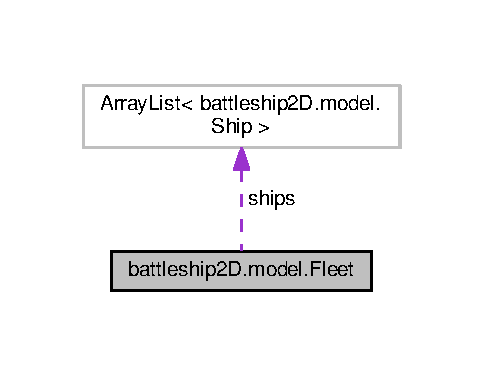
\includegraphics[width=232pt]{classbattleship2D_1_1model_1_1Fleet__coll__graph}
\end{center}
\end{figure}
\subsection*{Public Member Functions}
\begin{DoxyCompactItemize}
\item 
\hyperlink{classbattleship2D_1_1model_1_1Fleet_a9a46df779cb57eb0b1808a573ac4092b}{Fleet} ()
\begin{DoxyCompactList}\small\item\em Constructor. \end{DoxyCompactList}\item 
\hyperlink{classbattleship2D_1_1model_1_1Ship}{Ship} \hyperlink{classbattleship2D_1_1model_1_1Fleet_a7625af5c1f9ff69cdf36435071f68067}{find\-Ship\-From\-Type} (\hyperlink{enumbattleship2D_1_1model_1_1ShipType}{Ship\-Type} ship\-Type)
\item 
int \hyperlink{classbattleship2D_1_1model_1_1Fleet_a5a1b1a93de04523fbd611e8ab6409563}{number\-Of\-Ships} ()
\item 
void \hyperlink{classbattleship2D_1_1model_1_1Fleet_a0a3dc6a4439ff0cfee866ddea9f95dd6}{update\-Hits} (\hyperlink{enumbattleship2D_1_1model_1_1ShipType}{Ship\-Type} ship\-Type)
\begin{DoxyCompactList}\small\item\em Updates the number of ship parts that have been hit. \end{DoxyCompactList}\item 
Array\-List$<$ \hyperlink{classbattleship2D_1_1model_1_1Ship}{Ship} $>$ \hyperlink{classbattleship2D_1_1model_1_1Fleet_aba27f200100513da49d732f3f3f1a523}{get\-Ships} ()
\item 
Boolean \hyperlink{classbattleship2D_1_1model_1_1Fleet_ae00eeb3cee781f1a21886d8a51ee6ec6}{is\-Fleet\-Destroyed} ()
\item 
Boolean \hyperlink{classbattleship2D_1_1model_1_1Fleet_a441dbb2a73b4828fe232e800decbf93a}{is\-Last\-Hit\-Ship\-Destroyed} ()
\end{DoxyCompactItemize}
\subsection*{Private Member Functions}
\begin{DoxyCompactItemize}
\item 
void \hyperlink{classbattleship2D_1_1model_1_1Fleet_aed5a2244dee690f2640cc8d1960f0669}{init\-Remaining\-Parts} ()
\begin{DoxyCompactList}\small\item\em All ships are unscathed at first. \end{DoxyCompactList}\item 
void \hyperlink{classbattleship2D_1_1model_1_1Fleet_a554aa032fe5ad3811effe0acf8c47c18}{init\-Ships} ()
\begin{DoxyCompactList}\small\item\em Fills up the collection of ships. \end{DoxyCompactList}\item 
void \hyperlink{classbattleship2D_1_1model_1_1Fleet_a69efdd7a9a1fe25892d057f0f31c912f}{update\-Remaininghips} ()
\begin{DoxyCompactList}\small\item\em Updates fleet counters after a hit. \end{DoxyCompactList}\end{DoxyCompactItemize}
\subsection*{Private Attributes}
\begin{DoxyCompactItemize}
\item 
Boolean \hyperlink{classbattleship2D_1_1model_1_1Fleet_aa99ad6c0b52656c039a1b6e77d7a4f63}{fleet\-Destroyed} = false
\begin{DoxyCompactList}\small\item\em Checks whether the whole fleet has been destroyed. \end{DoxyCompactList}\item 
Boolean \hyperlink{classbattleship2D_1_1model_1_1Fleet_ac9245d7670e8ba55860fccead366b077}{last\-Hit\-Ship\-Destroyed} = false
\begin{DoxyCompactList}\small\item\em Checks whether the last hit ship has been entirely destroyed. \end{DoxyCompactList}\item 
final int\mbox{[}$\,$\mbox{]} \hyperlink{classbattleship2D_1_1model_1_1Fleet_acdbb1599e55f36117c255ee49df1148b}{remaining\-Parts}
\begin{DoxyCompactList}\small\item\em Counts ships parts which have not been hit. \end{DoxyCompactList}\item 
int \hyperlink{classbattleship2D_1_1model_1_1Fleet_a1e12ebdbc19e847806d5e41f69576cf7}{remaining\-Ships}
\begin{DoxyCompactList}\small\item\em Count still remaining ships. \end{DoxyCompactList}\item 
final Array\-List$<$ \hyperlink{classbattleship2D_1_1model_1_1Ship}{Ship} $>$ \hyperlink{classbattleship2D_1_1model_1_1Fleet_a969e704ee79c18874d9dddcf98401014}{ships}
\begin{DoxyCompactList}\small\item\em A fleet is made of different ships. \end{DoxyCompactList}\end{DoxyCompactItemize}


\subsection{Detailed Description}
\hyperlink{classbattleship2D_1_1model_1_1Fleet}{Fleet} of Ships. 

\begin{DoxyAuthor}{Author}
xaviator 
\end{DoxyAuthor}


\subsection{Constructor \& Destructor Documentation}
\hypertarget{classbattleship2D_1_1model_1_1Fleet_a9a46df779cb57eb0b1808a573ac4092b}{\index{battleship2\-D\-::model\-::\-Fleet@{battleship2\-D\-::model\-::\-Fleet}!Fleet@{Fleet}}
\index{Fleet@{Fleet}!battleship2D::model::Fleet@{battleship2\-D\-::model\-::\-Fleet}}
\subsubsection[{Fleet}]{\setlength{\rightskip}{0pt plus 5cm}battleship2\-D.\-model.\-Fleet.\-Fleet (
\begin{DoxyParamCaption}
{}
\end{DoxyParamCaption}
)}}\label{classbattleship2D_1_1model_1_1Fleet_a9a46df779cb57eb0b1808a573ac4092b}


Constructor. 



\subsection{Member Function Documentation}
\hypertarget{classbattleship2D_1_1model_1_1Fleet_a7625af5c1f9ff69cdf36435071f68067}{\index{battleship2\-D\-::model\-::\-Fleet@{battleship2\-D\-::model\-::\-Fleet}!find\-Ship\-From\-Type@{find\-Ship\-From\-Type}}
\index{find\-Ship\-From\-Type@{find\-Ship\-From\-Type}!battleship2D::model::Fleet@{battleship2\-D\-::model\-::\-Fleet}}
\subsubsection[{find\-Ship\-From\-Type}]{\setlength{\rightskip}{0pt plus 5cm}{\bf Ship} battleship2\-D.\-model.\-Fleet.\-find\-Ship\-From\-Type (
\begin{DoxyParamCaption}
\item[{{\bf Ship\-Type}}]{ship\-Type}
\end{DoxyParamCaption}
)}}\label{classbattleship2D_1_1model_1_1Fleet_a7625af5c1f9ff69cdf36435071f68067}

\begin{DoxyParams}{Parameters}
{\em ship\-Type} & -\/ type of the ship to find \\
\hline
\end{DoxyParams}
\begin{DoxyReturn}{Returns}
the ship matching shiptype, null otherwise 
\end{DoxyReturn}
\hypertarget{classbattleship2D_1_1model_1_1Fleet_aba27f200100513da49d732f3f3f1a523}{\index{battleship2\-D\-::model\-::\-Fleet@{battleship2\-D\-::model\-::\-Fleet}!get\-Ships@{get\-Ships}}
\index{get\-Ships@{get\-Ships}!battleship2D::model::Fleet@{battleship2\-D\-::model\-::\-Fleet}}
\subsubsection[{get\-Ships}]{\setlength{\rightskip}{0pt plus 5cm}Array\-List$<${\bf Ship}$>$ battleship2\-D.\-model.\-Fleet.\-get\-Ships (
\begin{DoxyParamCaption}
{}
\end{DoxyParamCaption}
)}}\label{classbattleship2D_1_1model_1_1Fleet_aba27f200100513da49d732f3f3f1a523}
\hypertarget{classbattleship2D_1_1model_1_1Fleet_aed5a2244dee690f2640cc8d1960f0669}{\index{battleship2\-D\-::model\-::\-Fleet@{battleship2\-D\-::model\-::\-Fleet}!init\-Remaining\-Parts@{init\-Remaining\-Parts}}
\index{init\-Remaining\-Parts@{init\-Remaining\-Parts}!battleship2D::model::Fleet@{battleship2\-D\-::model\-::\-Fleet}}
\subsubsection[{init\-Remaining\-Parts}]{\setlength{\rightskip}{0pt plus 5cm}void battleship2\-D.\-model.\-Fleet.\-init\-Remaining\-Parts (
\begin{DoxyParamCaption}
{}
\end{DoxyParamCaption}
)\hspace{0.3cm}{\ttfamily [private]}}}\label{classbattleship2D_1_1model_1_1Fleet_aed5a2244dee690f2640cc8d1960f0669}


All ships are unscathed at first. 

\begin{DoxySeeAlso}{See Also}
\hyperlink{classbattleship2D_1_1model_1_1Fleet_a9a46df779cb57eb0b1808a573ac4092b}{Fleet()} 
\end{DoxySeeAlso}
\hypertarget{classbattleship2D_1_1model_1_1Fleet_a554aa032fe5ad3811effe0acf8c47c18}{\index{battleship2\-D\-::model\-::\-Fleet@{battleship2\-D\-::model\-::\-Fleet}!init\-Ships@{init\-Ships}}
\index{init\-Ships@{init\-Ships}!battleship2D::model::Fleet@{battleship2\-D\-::model\-::\-Fleet}}
\subsubsection[{init\-Ships}]{\setlength{\rightskip}{0pt plus 5cm}void battleship2\-D.\-model.\-Fleet.\-init\-Ships (
\begin{DoxyParamCaption}
{}
\end{DoxyParamCaption}
)\hspace{0.3cm}{\ttfamily [private]}}}\label{classbattleship2D_1_1model_1_1Fleet_a554aa032fe5ad3811effe0acf8c47c18}


Fills up the collection of ships. 

\begin{DoxySeeAlso}{See Also}
\hyperlink{classbattleship2D_1_1model_1_1Fleet_a9a46df779cb57eb0b1808a573ac4092b}{Fleet()} 
\end{DoxySeeAlso}
\hypertarget{classbattleship2D_1_1model_1_1Fleet_ae00eeb3cee781f1a21886d8a51ee6ec6}{\index{battleship2\-D\-::model\-::\-Fleet@{battleship2\-D\-::model\-::\-Fleet}!is\-Fleet\-Destroyed@{is\-Fleet\-Destroyed}}
\index{is\-Fleet\-Destroyed@{is\-Fleet\-Destroyed}!battleship2D::model::Fleet@{battleship2\-D\-::model\-::\-Fleet}}
\subsubsection[{is\-Fleet\-Destroyed}]{\setlength{\rightskip}{0pt plus 5cm}Boolean battleship2\-D.\-model.\-Fleet.\-is\-Fleet\-Destroyed (
\begin{DoxyParamCaption}
{}
\end{DoxyParamCaption}
)}}\label{classbattleship2D_1_1model_1_1Fleet_ae00eeb3cee781f1a21886d8a51ee6ec6}
\hypertarget{classbattleship2D_1_1model_1_1Fleet_a441dbb2a73b4828fe232e800decbf93a}{\index{battleship2\-D\-::model\-::\-Fleet@{battleship2\-D\-::model\-::\-Fleet}!is\-Last\-Hit\-Ship\-Destroyed@{is\-Last\-Hit\-Ship\-Destroyed}}
\index{is\-Last\-Hit\-Ship\-Destroyed@{is\-Last\-Hit\-Ship\-Destroyed}!battleship2D::model::Fleet@{battleship2\-D\-::model\-::\-Fleet}}
\subsubsection[{is\-Last\-Hit\-Ship\-Destroyed}]{\setlength{\rightskip}{0pt plus 5cm}Boolean battleship2\-D.\-model.\-Fleet.\-is\-Last\-Hit\-Ship\-Destroyed (
\begin{DoxyParamCaption}
{}
\end{DoxyParamCaption}
)}}\label{classbattleship2D_1_1model_1_1Fleet_a441dbb2a73b4828fe232e800decbf93a}
\hypertarget{classbattleship2D_1_1model_1_1Fleet_a5a1b1a93de04523fbd611e8ab6409563}{\index{battleship2\-D\-::model\-::\-Fleet@{battleship2\-D\-::model\-::\-Fleet}!number\-Of\-Ships@{number\-Of\-Ships}}
\index{number\-Of\-Ships@{number\-Of\-Ships}!battleship2D::model::Fleet@{battleship2\-D\-::model\-::\-Fleet}}
\subsubsection[{number\-Of\-Ships}]{\setlength{\rightskip}{0pt plus 5cm}int battleship2\-D.\-model.\-Fleet.\-number\-Of\-Ships (
\begin{DoxyParamCaption}
{}
\end{DoxyParamCaption}
)}}\label{classbattleship2D_1_1model_1_1Fleet_a5a1b1a93de04523fbd611e8ab6409563}
\begin{DoxyReturn}{Returns}
the number of ships in the fleet 
\end{DoxyReturn}
\hypertarget{classbattleship2D_1_1model_1_1Fleet_a0a3dc6a4439ff0cfee866ddea9f95dd6}{\index{battleship2\-D\-::model\-::\-Fleet@{battleship2\-D\-::model\-::\-Fleet}!update\-Hits@{update\-Hits}}
\index{update\-Hits@{update\-Hits}!battleship2D::model::Fleet@{battleship2\-D\-::model\-::\-Fleet}}
\subsubsection[{update\-Hits}]{\setlength{\rightskip}{0pt plus 5cm}void battleship2\-D.\-model.\-Fleet.\-update\-Hits (
\begin{DoxyParamCaption}
\item[{{\bf Ship\-Type}}]{ship\-Type}
\end{DoxyParamCaption}
)}}\label{classbattleship2D_1_1model_1_1Fleet_a0a3dc6a4439ff0cfee866ddea9f95dd6}


Updates the number of ship parts that have been hit. 


\begin{DoxyParams}{Parameters}
{\em ship\-Type} & -\/ type of the ship to deal with \\
\hline
\end{DoxyParams}
\hypertarget{classbattleship2D_1_1model_1_1Fleet_a69efdd7a9a1fe25892d057f0f31c912f}{\index{battleship2\-D\-::model\-::\-Fleet@{battleship2\-D\-::model\-::\-Fleet}!update\-Remaininghips@{update\-Remaininghips}}
\index{update\-Remaininghips@{update\-Remaininghips}!battleship2D::model::Fleet@{battleship2\-D\-::model\-::\-Fleet}}
\subsubsection[{update\-Remaininghips}]{\setlength{\rightskip}{0pt plus 5cm}void battleship2\-D.\-model.\-Fleet.\-update\-Remaininghips (
\begin{DoxyParamCaption}
{}
\end{DoxyParamCaption}
)\hspace{0.3cm}{\ttfamily [private]}}}\label{classbattleship2D_1_1model_1_1Fleet_a69efdd7a9a1fe25892d057f0f31c912f}


Updates fleet counters after a hit. 

\begin{DoxySeeAlso}{See Also}
\hyperlink{classbattleship2D_1_1model_1_1Fleet_a0a3dc6a4439ff0cfee866ddea9f95dd6}{update\-Hits()} 
\end{DoxySeeAlso}


\subsection{Member Data Documentation}
\hypertarget{classbattleship2D_1_1model_1_1Fleet_aa99ad6c0b52656c039a1b6e77d7a4f63}{\index{battleship2\-D\-::model\-::\-Fleet@{battleship2\-D\-::model\-::\-Fleet}!fleet\-Destroyed@{fleet\-Destroyed}}
\index{fleet\-Destroyed@{fleet\-Destroyed}!battleship2D::model::Fleet@{battleship2\-D\-::model\-::\-Fleet}}
\subsubsection[{fleet\-Destroyed}]{\setlength{\rightskip}{0pt plus 5cm}Boolean battleship2\-D.\-model.\-Fleet.\-fleet\-Destroyed = false\hspace{0.3cm}{\ttfamily [private]}}}\label{classbattleship2D_1_1model_1_1Fleet_aa99ad6c0b52656c039a1b6e77d7a4f63}


Checks whether the whole fleet has been destroyed. 

\hypertarget{classbattleship2D_1_1model_1_1Fleet_ac9245d7670e8ba55860fccead366b077}{\index{battleship2\-D\-::model\-::\-Fleet@{battleship2\-D\-::model\-::\-Fleet}!last\-Hit\-Ship\-Destroyed@{last\-Hit\-Ship\-Destroyed}}
\index{last\-Hit\-Ship\-Destroyed@{last\-Hit\-Ship\-Destroyed}!battleship2D::model::Fleet@{battleship2\-D\-::model\-::\-Fleet}}
\subsubsection[{last\-Hit\-Ship\-Destroyed}]{\setlength{\rightskip}{0pt plus 5cm}Boolean battleship2\-D.\-model.\-Fleet.\-last\-Hit\-Ship\-Destroyed = false\hspace{0.3cm}{\ttfamily [private]}}}\label{classbattleship2D_1_1model_1_1Fleet_ac9245d7670e8ba55860fccead366b077}


Checks whether the last hit ship has been entirely destroyed. 

\hypertarget{classbattleship2D_1_1model_1_1Fleet_acdbb1599e55f36117c255ee49df1148b}{\index{battleship2\-D\-::model\-::\-Fleet@{battleship2\-D\-::model\-::\-Fleet}!remaining\-Parts@{remaining\-Parts}}
\index{remaining\-Parts@{remaining\-Parts}!battleship2D::model::Fleet@{battleship2\-D\-::model\-::\-Fleet}}
\subsubsection[{remaining\-Parts}]{\setlength{\rightskip}{0pt plus 5cm}final int \mbox{[}$\,$\mbox{]} battleship2\-D.\-model.\-Fleet.\-remaining\-Parts\hspace{0.3cm}{\ttfamily [private]}}}\label{classbattleship2D_1_1model_1_1Fleet_acdbb1599e55f36117c255ee49df1148b}


Counts ships parts which have not been hit. 

\hypertarget{classbattleship2D_1_1model_1_1Fleet_a1e12ebdbc19e847806d5e41f69576cf7}{\index{battleship2\-D\-::model\-::\-Fleet@{battleship2\-D\-::model\-::\-Fleet}!remaining\-Ships@{remaining\-Ships}}
\index{remaining\-Ships@{remaining\-Ships}!battleship2D::model::Fleet@{battleship2\-D\-::model\-::\-Fleet}}
\subsubsection[{remaining\-Ships}]{\setlength{\rightskip}{0pt plus 5cm}int battleship2\-D.\-model.\-Fleet.\-remaining\-Ships\hspace{0.3cm}{\ttfamily [private]}}}\label{classbattleship2D_1_1model_1_1Fleet_a1e12ebdbc19e847806d5e41f69576cf7}


Count still remaining ships. 

\hypertarget{classbattleship2D_1_1model_1_1Fleet_a969e704ee79c18874d9dddcf98401014}{\index{battleship2\-D\-::model\-::\-Fleet@{battleship2\-D\-::model\-::\-Fleet}!ships@{ships}}
\index{ships@{ships}!battleship2D::model::Fleet@{battleship2\-D\-::model\-::\-Fleet}}
\subsubsection[{ships}]{\setlength{\rightskip}{0pt plus 5cm}final Array\-List$<${\bf Ship}$>$ battleship2\-D.\-model.\-Fleet.\-ships\hspace{0.3cm}{\ttfamily [private]}}}\label{classbattleship2D_1_1model_1_1Fleet_a969e704ee79c18874d9dddcf98401014}


A fleet is made of different ships. 



The documentation for this class was generated from the following file\-:\begin{DoxyCompactItemize}
\item 
/home/xaviator/\-Enseignements/2015-\/2016/\-S\-F\-A/\-M1-\/\-Info/\-I\-H\-M/\-Battle\-Ship2\-D\-\_\-students/battleship2\-D/model/\hyperlink{Fleet_8java}{Fleet.\-java}\end{DoxyCompactItemize}

\hypertarget{classbattleship2D_1_1model_1_1Ship}{\section{battleship2\-D.\-model.\-Ship Class Reference}
\label{classbattleship2D_1_1model_1_1Ship}\index{battleship2\-D.\-model.\-Ship@{battleship2\-D.\-model.\-Ship}}
}


\hyperlink{classbattleship2D_1_1model_1_1Ship}{Ship} representation on the board A ship is made of tiles aligned along either the X-\/axis or the Y-\/axis.  




Collaboration diagram for battleship2\-D.\-model.\-Ship\-:\nopagebreak
\begin{figure}[H]
\begin{center}
\leavevmode
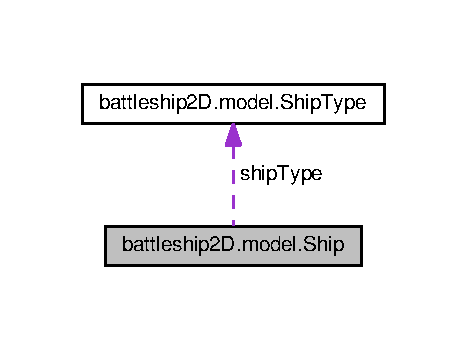
\includegraphics[width=224pt]{classbattleship2D_1_1model_1_1Ship__coll__graph}
\end{center}
\end{figure}
\subsection*{Public Member Functions}
\begin{DoxyCompactItemize}
\item 
\hyperlink{classbattleship2D_1_1model_1_1Ship_a87eba7afe7524d43b60439a5fd269009}{Ship} (\hyperlink{enumbattleship2D_1_1model_1_1ShipType}{Ship\-Type} \hyperlink{classbattleship2D_1_1model_1_1Ship_a9291fcd44b67561c908b6c7e47dc844f}{ship\-Type})
\begin{DoxyCompactList}\small\item\em Constructor. \end{DoxyCompactList}\item 
int \hyperlink{classbattleship2D_1_1model_1_1Ship_ab572418d97ac961f1a6e59f7ea082a99}{get\-Size} ()
\item 
\hyperlink{enumbattleship2D_1_1model_1_1ShipType}{Ship\-Type} \hyperlink{classbattleship2D_1_1model_1_1Ship_a6fccc3e46fdcf915a65e2e51d0da91c6}{get\-Ship\-Type} ()
\item 
String \hyperlink{classbattleship2D_1_1model_1_1Ship_acf78dc2817640d57af66e296f3072123}{get\-Description} ()
\end{DoxyCompactItemize}
\subsection*{Private Member Functions}
\begin{DoxyCompactItemize}
\item 
void \hyperlink{classbattleship2D_1_1model_1_1Ship_a677853c8501c31c34d69788df6c1c49d}{init\-Ship} ()
\begin{DoxyCompactList}\small\item\em Sets \hyperlink{classbattleship2D_1_1model_1_1Ship}{Ship}'s characteristics. \end{DoxyCompactList}\end{DoxyCompactItemize}
\subsection*{Private Attributes}
\begin{DoxyCompactItemize}
\item 
String \hyperlink{classbattleship2D_1_1model_1_1Ship_a902a3f9c168d56cc3c8d95747e133a3c}{description}
\begin{DoxyCompactList}\small\item\em Short description. \end{DoxyCompactList}\item 
final \hyperlink{enumbattleship2D_1_1model_1_1ShipType}{Ship\-Type} \hyperlink{classbattleship2D_1_1model_1_1Ship_a9291fcd44b67561c908b6c7e47dc844f}{ship\-Type}
\begin{DoxyCompactList}\small\item\em \hyperlink{classbattleship2D_1_1model_1_1Ship}{Ship}'s type. \end{DoxyCompactList}\item 
int \hyperlink{classbattleship2D_1_1model_1_1Ship_a8c1f963c60a57e54b2600e9ee3a5aef6}{size}
\begin{DoxyCompactList}\small\item\em \hyperlink{classbattleship2D_1_1model_1_1Ship}{Ship}'s size in cells. \end{DoxyCompactList}\end{DoxyCompactItemize}


\subsection{Detailed Description}
\hyperlink{classbattleship2D_1_1model_1_1Ship}{Ship} representation on the board A ship is made of tiles aligned along either the X-\/axis or the Y-\/axis. 

\begin{DoxyAuthor}{Author}
xaviator 
\end{DoxyAuthor}


\subsection{Constructor \& Destructor Documentation}
\hypertarget{classbattleship2D_1_1model_1_1Ship_a87eba7afe7524d43b60439a5fd269009}{\index{battleship2\-D\-::model\-::\-Ship@{battleship2\-D\-::model\-::\-Ship}!Ship@{Ship}}
\index{Ship@{Ship}!battleship2D::model::Ship@{battleship2\-D\-::model\-::\-Ship}}
\subsubsection[{Ship}]{\setlength{\rightskip}{0pt plus 5cm}battleship2\-D.\-model.\-Ship.\-Ship (
\begin{DoxyParamCaption}
\item[{{\bf Ship\-Type}}]{ship\-Type}
\end{DoxyParamCaption}
)}}\label{classbattleship2D_1_1model_1_1Ship_a87eba7afe7524d43b60439a5fd269009}


Constructor. 


\begin{DoxyParams}{Parameters}
{\em ship\-Type} & ship's type \\
\hline
\end{DoxyParams}


\subsection{Member Function Documentation}
\hypertarget{classbattleship2D_1_1model_1_1Ship_acf78dc2817640d57af66e296f3072123}{\index{battleship2\-D\-::model\-::\-Ship@{battleship2\-D\-::model\-::\-Ship}!get\-Description@{get\-Description}}
\index{get\-Description@{get\-Description}!battleship2D::model::Ship@{battleship2\-D\-::model\-::\-Ship}}
\subsubsection[{get\-Description}]{\setlength{\rightskip}{0pt plus 5cm}String battleship2\-D.\-model.\-Ship.\-get\-Description (
\begin{DoxyParamCaption}
{}
\end{DoxyParamCaption}
)}}\label{classbattleship2D_1_1model_1_1Ship_acf78dc2817640d57af66e296f3072123}
\hypertarget{classbattleship2D_1_1model_1_1Ship_a6fccc3e46fdcf915a65e2e51d0da91c6}{\index{battleship2\-D\-::model\-::\-Ship@{battleship2\-D\-::model\-::\-Ship}!get\-Ship\-Type@{get\-Ship\-Type}}
\index{get\-Ship\-Type@{get\-Ship\-Type}!battleship2D::model::Ship@{battleship2\-D\-::model\-::\-Ship}}
\subsubsection[{get\-Ship\-Type}]{\setlength{\rightskip}{0pt plus 5cm}{\bf Ship\-Type} battleship2\-D.\-model.\-Ship.\-get\-Ship\-Type (
\begin{DoxyParamCaption}
{}
\end{DoxyParamCaption}
)}}\label{classbattleship2D_1_1model_1_1Ship_a6fccc3e46fdcf915a65e2e51d0da91c6}
\hypertarget{classbattleship2D_1_1model_1_1Ship_ab572418d97ac961f1a6e59f7ea082a99}{\index{battleship2\-D\-::model\-::\-Ship@{battleship2\-D\-::model\-::\-Ship}!get\-Size@{get\-Size}}
\index{get\-Size@{get\-Size}!battleship2D::model::Ship@{battleship2\-D\-::model\-::\-Ship}}
\subsubsection[{get\-Size}]{\setlength{\rightskip}{0pt plus 5cm}int battleship2\-D.\-model.\-Ship.\-get\-Size (
\begin{DoxyParamCaption}
{}
\end{DoxyParamCaption}
)}}\label{classbattleship2D_1_1model_1_1Ship_ab572418d97ac961f1a6e59f7ea082a99}
\hypertarget{classbattleship2D_1_1model_1_1Ship_a677853c8501c31c34d69788df6c1c49d}{\index{battleship2\-D\-::model\-::\-Ship@{battleship2\-D\-::model\-::\-Ship}!init\-Ship@{init\-Ship}}
\index{init\-Ship@{init\-Ship}!battleship2D::model::Ship@{battleship2\-D\-::model\-::\-Ship}}
\subsubsection[{init\-Ship}]{\setlength{\rightskip}{0pt plus 5cm}void battleship2\-D.\-model.\-Ship.\-init\-Ship (
\begin{DoxyParamCaption}
{}
\end{DoxyParamCaption}
)\hspace{0.3cm}{\ttfamily [private]}}}\label{classbattleship2D_1_1model_1_1Ship_a677853c8501c31c34d69788df6c1c49d}


Sets \hyperlink{classbattleship2D_1_1model_1_1Ship}{Ship}'s characteristics. 

\begin{DoxySeeAlso}{See Also}
\hyperlink{classbattleship2D_1_1model_1_1Ship_a87eba7afe7524d43b60439a5fd269009}{Ship()} 
\end{DoxySeeAlso}


\subsection{Member Data Documentation}
\hypertarget{classbattleship2D_1_1model_1_1Ship_a902a3f9c168d56cc3c8d95747e133a3c}{\index{battleship2\-D\-::model\-::\-Ship@{battleship2\-D\-::model\-::\-Ship}!description@{description}}
\index{description@{description}!battleship2D::model::Ship@{battleship2\-D\-::model\-::\-Ship}}
\subsubsection[{description}]{\setlength{\rightskip}{0pt plus 5cm}String battleship2\-D.\-model.\-Ship.\-description\hspace{0.3cm}{\ttfamily [private]}}}\label{classbattleship2D_1_1model_1_1Ship_a902a3f9c168d56cc3c8d95747e133a3c}


Short description. 

\hypertarget{classbattleship2D_1_1model_1_1Ship_a9291fcd44b67561c908b6c7e47dc844f}{\index{battleship2\-D\-::model\-::\-Ship@{battleship2\-D\-::model\-::\-Ship}!ship\-Type@{ship\-Type}}
\index{ship\-Type@{ship\-Type}!battleship2D::model::Ship@{battleship2\-D\-::model\-::\-Ship}}
\subsubsection[{ship\-Type}]{\setlength{\rightskip}{0pt plus 5cm}final {\bf Ship\-Type} battleship2\-D.\-model.\-Ship.\-ship\-Type\hspace{0.3cm}{\ttfamily [private]}}}\label{classbattleship2D_1_1model_1_1Ship_a9291fcd44b67561c908b6c7e47dc844f}


\hyperlink{classbattleship2D_1_1model_1_1Ship}{Ship}'s type. 

\hypertarget{classbattleship2D_1_1model_1_1Ship_a8c1f963c60a57e54b2600e9ee3a5aef6}{\index{battleship2\-D\-::model\-::\-Ship@{battleship2\-D\-::model\-::\-Ship}!size@{size}}
\index{size@{size}!battleship2D::model::Ship@{battleship2\-D\-::model\-::\-Ship}}
\subsubsection[{size}]{\setlength{\rightskip}{0pt plus 5cm}int battleship2\-D.\-model.\-Ship.\-size\hspace{0.3cm}{\ttfamily [private]}}}\label{classbattleship2D_1_1model_1_1Ship_a8c1f963c60a57e54b2600e9ee3a5aef6}


\hyperlink{classbattleship2D_1_1model_1_1Ship}{Ship}'s size in cells. 



The documentation for this class was generated from the following file\-:\begin{DoxyCompactItemize}
\item 
/home/xaviator/\-Enseignements/2015-\/2016/\-S\-F\-A/\-M1-\/\-Info/\-I\-H\-M/\-Battle\-Ship2\-D\-\_\-students/battleship2\-D/model/\hyperlink{Ship_8java}{Ship.\-java}\end{DoxyCompactItemize}

\hypertarget{enumbattleship2D_1_1model_1_1ShipType}{\section{battleship2\-D.\-model.\-Ship\-Type Enum Reference}
\label{enumbattleship2D_1_1model_1_1ShipType}\index{battleship2\-D.\-model.\-Ship\-Type@{battleship2\-D.\-model.\-Ship\-Type}}
}


\hyperlink{classbattleship2D_1_1model_1_1Ship}{Ship} types.  


\subsection*{Public Member Functions}
\begin{DoxyCompactItemize}
\item 
String \hyperlink{enumbattleship2D_1_1model_1_1ShipType_a76b27b28d4fc80ce17e5d3e3370281a0}{get\-Description} ()
\item 
String \hyperlink{enumbattleship2D_1_1model_1_1ShipType_ae18e6c6a04dfc1bf3aaca096c545921a}{get\-Appearance} ()
\end{DoxyCompactItemize}
\subsection*{Public Attributes}
\begin{DoxyCompactItemize}
\item 
\hyperlink{enumbattleship2D_1_1model_1_1ShipType_ab3cfa603543cb285e992850a6f7c954d}{B\-A\-T\-T\-L\-E\-S\-H\-I\-P} =(\char`\"{}Battleship\char`\"{}, \char`\"{}-\/fx-\/background-\/image\-: url(\textbackslash{}\char`\"{}battleship2\-D/pictures/battleship.\-jpg\textbackslash{}\char`\"{})\char`\"{})
\item 
\hyperlink{enumbattleship2D_1_1model_1_1ShipType_ab24d6f8e734fcdb708100c0ae4aaaf50}{C\-A\-R\-R\-I\-E\-R} =(\char`\"{}Carrier\char`\"{}, \char`\"{}-\/fx-\/background-\/image\-: url(\textbackslash{}\char`\"{}battleship2\-D/pictures/carrier.\-jpg\textbackslash{}\char`\"{})\char`\"{})
\item 
\hyperlink{enumbattleship2D_1_1model_1_1ShipType_ae1b8a67f35620be66e722436cc116a03}{C\-R\-U\-I\-S\-E\-R} =(\char`\"{}Cruiser\char`\"{}, \char`\"{}-\/fx-\/background-\/image\-: url(\textbackslash{}\char`\"{}battleship2\-D/pictures/cruiser.\-jpg\textbackslash{}\char`\"{})\char`\"{})
\item 
\hyperlink{enumbattleship2D_1_1model_1_1ShipType_afb73a729348c4ae84ea2e4d2ff1160de}{D\-E\-S\-T\-R\-O\-Y\-E\-R} =(\char`\"{}Destroyer\char`\"{}, \char`\"{}-\/fx-\/background-\/image\-: url(\textbackslash{}\char`\"{}battleship2\-D/pictures/destroyer.\-jpg\textbackslash{}\char`\"{})\char`\"{})
\item 
\hyperlink{enumbattleship2D_1_1model_1_1ShipType_a6a4a2e419cb22ff18555e82539251a9d}{S\-U\-B\-M\-A\-R\-I\-N\-E} =(\char`\"{}Submarine\char`\"{}, \char`\"{}-\/fx-\/background-\/image\-: url(\textbackslash{}\char`\"{}battleship2\-D/pictures/submarine.\-jpeg\textbackslash{}\char`\"{})\char`\"{})
\end{DoxyCompactItemize}
\subsection*{Private Member Functions}
\begin{DoxyCompactItemize}
\item 
\hyperlink{enumbattleship2D_1_1model_1_1ShipType_af75a4ecff25c2d6fd086c0f9e443d8ab}{Ship\-Type} (final String \hyperlink{enumbattleship2D_1_1model_1_1ShipType_a99b2dcefbf9c3c0c210d2f7760d247ef}{description}, final String \hyperlink{enumbattleship2D_1_1model_1_1ShipType_a003ee9ae1371b0c5ad31c39d2653b850}{appearance})
\begin{DoxyCompactList}\small\item\em Constructor. \end{DoxyCompactList}\end{DoxyCompactItemize}
\subsection*{Private Attributes}
\begin{DoxyCompactItemize}
\item 
final String \hyperlink{enumbattleship2D_1_1model_1_1ShipType_a003ee9ae1371b0c5ad31c39d2653b850}{appearance}
\begin{DoxyCompactList}\small\item\em Rendering either as a color or an image. \end{DoxyCompactList}\item 
final String \hyperlink{enumbattleship2D_1_1model_1_1ShipType_a99b2dcefbf9c3c0c210d2f7760d247ef}{description}
\begin{DoxyCompactList}\small\item\em Short description. \end{DoxyCompactList}\end{DoxyCompactItemize}


\subsection{Detailed Description}
\hyperlink{classbattleship2D_1_1model_1_1Ship}{Ship} types. 

\begin{DoxyAuthor}{Author}
xaviator 
\end{DoxyAuthor}


\subsection{Constructor \& Destructor Documentation}
\hypertarget{enumbattleship2D_1_1model_1_1ShipType_af75a4ecff25c2d6fd086c0f9e443d8ab}{\index{battleship2\-D\-::model\-::\-Ship\-Type@{battleship2\-D\-::model\-::\-Ship\-Type}!Ship\-Type@{Ship\-Type}}
\index{Ship\-Type@{Ship\-Type}!battleship2D::model::ShipType@{battleship2\-D\-::model\-::\-Ship\-Type}}
\subsubsection[{Ship\-Type}]{\setlength{\rightskip}{0pt plus 5cm}battleship2\-D.\-model.\-Ship\-Type.\-Ship\-Type (
\begin{DoxyParamCaption}
\item[{final String}]{description, }
\item[{final String}]{appearance}
\end{DoxyParamCaption}
)\hspace{0.3cm}{\ttfamily [private]}}}\label{enumbattleship2D_1_1model_1_1ShipType_af75a4ecff25c2d6fd086c0f9e443d8ab}


Constructor. 


\begin{DoxyParams}{Parameters}
{\em description} & -\/ short description \\
\hline
{\em color} & -\/ related color \\
\hline
\end{DoxyParams}


\subsection{Member Function Documentation}
\hypertarget{enumbattleship2D_1_1model_1_1ShipType_ae18e6c6a04dfc1bf3aaca096c545921a}{\index{battleship2\-D\-::model\-::\-Ship\-Type@{battleship2\-D\-::model\-::\-Ship\-Type}!get\-Appearance@{get\-Appearance}}
\index{get\-Appearance@{get\-Appearance}!battleship2D::model::ShipType@{battleship2\-D\-::model\-::\-Ship\-Type}}
\subsubsection[{get\-Appearance}]{\setlength{\rightskip}{0pt plus 5cm}String battleship2\-D.\-model.\-Ship\-Type.\-get\-Appearance (
\begin{DoxyParamCaption}
{}
\end{DoxyParamCaption}
)}}\label{enumbattleship2D_1_1model_1_1ShipType_ae18e6c6a04dfc1bf3aaca096c545921a}
\begin{DoxyReturn}{Returns}
the appearance field 
\end{DoxyReturn}
\hypertarget{enumbattleship2D_1_1model_1_1ShipType_a76b27b28d4fc80ce17e5d3e3370281a0}{\index{battleship2\-D\-::model\-::\-Ship\-Type@{battleship2\-D\-::model\-::\-Ship\-Type}!get\-Description@{get\-Description}}
\index{get\-Description@{get\-Description}!battleship2D::model::ShipType@{battleship2\-D\-::model\-::\-Ship\-Type}}
\subsubsection[{get\-Description}]{\setlength{\rightskip}{0pt plus 5cm}String battleship2\-D.\-model.\-Ship\-Type.\-get\-Description (
\begin{DoxyParamCaption}
{}
\end{DoxyParamCaption}
)}}\label{enumbattleship2D_1_1model_1_1ShipType_a76b27b28d4fc80ce17e5d3e3370281a0}
\begin{DoxyReturn}{Returns}
the description field 
\end{DoxyReturn}


\subsection{Member Data Documentation}
\hypertarget{enumbattleship2D_1_1model_1_1ShipType_a003ee9ae1371b0c5ad31c39d2653b850}{\index{battleship2\-D\-::model\-::\-Ship\-Type@{battleship2\-D\-::model\-::\-Ship\-Type}!appearance@{appearance}}
\index{appearance@{appearance}!battleship2D::model::ShipType@{battleship2\-D\-::model\-::\-Ship\-Type}}
\subsubsection[{appearance}]{\setlength{\rightskip}{0pt plus 5cm}final String battleship2\-D.\-model.\-Ship\-Type.\-appearance\hspace{0.3cm}{\ttfamily [private]}}}\label{enumbattleship2D_1_1model_1_1ShipType_a003ee9ae1371b0c5ad31c39d2653b850}


Rendering either as a color or an image. 

\hypertarget{enumbattleship2D_1_1model_1_1ShipType_ab3cfa603543cb285e992850a6f7c954d}{\index{battleship2\-D\-::model\-::\-Ship\-Type@{battleship2\-D\-::model\-::\-Ship\-Type}!B\-A\-T\-T\-L\-E\-S\-H\-I\-P@{B\-A\-T\-T\-L\-E\-S\-H\-I\-P}}
\index{B\-A\-T\-T\-L\-E\-S\-H\-I\-P@{B\-A\-T\-T\-L\-E\-S\-H\-I\-P}!battleship2D::model::ShipType@{battleship2\-D\-::model\-::\-Ship\-Type}}
\subsubsection[{B\-A\-T\-T\-L\-E\-S\-H\-I\-P}]{\setlength{\rightskip}{0pt plus 5cm}battleship2\-D.\-model.\-Ship\-Type.\-B\-A\-T\-T\-L\-E\-S\-H\-I\-P =(\char`\"{}Battleship\char`\"{}, \char`\"{}-\/fx-\/background-\/image\-: url(\textbackslash{}\char`\"{}battleship2\-D/pictures/battleship.\-jpg\textbackslash{}\char`\"{})\char`\"{})}}\label{enumbattleship2D_1_1model_1_1ShipType_ab3cfa603543cb285e992850a6f7c954d}
\hypertarget{enumbattleship2D_1_1model_1_1ShipType_ab24d6f8e734fcdb708100c0ae4aaaf50}{\index{battleship2\-D\-::model\-::\-Ship\-Type@{battleship2\-D\-::model\-::\-Ship\-Type}!C\-A\-R\-R\-I\-E\-R@{C\-A\-R\-R\-I\-E\-R}}
\index{C\-A\-R\-R\-I\-E\-R@{C\-A\-R\-R\-I\-E\-R}!battleship2D::model::ShipType@{battleship2\-D\-::model\-::\-Ship\-Type}}
\subsubsection[{C\-A\-R\-R\-I\-E\-R}]{\setlength{\rightskip}{0pt plus 5cm}battleship2\-D.\-model.\-Ship\-Type.\-C\-A\-R\-R\-I\-E\-R =(\char`\"{}Carrier\char`\"{}, \char`\"{}-\/fx-\/background-\/image\-: url(\textbackslash{}\char`\"{}battleship2\-D/pictures/carrier.\-jpg\textbackslash{}\char`\"{})\char`\"{})}}\label{enumbattleship2D_1_1model_1_1ShipType_ab24d6f8e734fcdb708100c0ae4aaaf50}
\hypertarget{enumbattleship2D_1_1model_1_1ShipType_ae1b8a67f35620be66e722436cc116a03}{\index{battleship2\-D\-::model\-::\-Ship\-Type@{battleship2\-D\-::model\-::\-Ship\-Type}!C\-R\-U\-I\-S\-E\-R@{C\-R\-U\-I\-S\-E\-R}}
\index{C\-R\-U\-I\-S\-E\-R@{C\-R\-U\-I\-S\-E\-R}!battleship2D::model::ShipType@{battleship2\-D\-::model\-::\-Ship\-Type}}
\subsubsection[{C\-R\-U\-I\-S\-E\-R}]{\setlength{\rightskip}{0pt plus 5cm}battleship2\-D.\-model.\-Ship\-Type.\-C\-R\-U\-I\-S\-E\-R =(\char`\"{}Cruiser\char`\"{}, \char`\"{}-\/fx-\/background-\/image\-: url(\textbackslash{}\char`\"{}battleship2\-D/pictures/cruiser.\-jpg\textbackslash{}\char`\"{})\char`\"{})}}\label{enumbattleship2D_1_1model_1_1ShipType_ae1b8a67f35620be66e722436cc116a03}
\hypertarget{enumbattleship2D_1_1model_1_1ShipType_a99b2dcefbf9c3c0c210d2f7760d247ef}{\index{battleship2\-D\-::model\-::\-Ship\-Type@{battleship2\-D\-::model\-::\-Ship\-Type}!description@{description}}
\index{description@{description}!battleship2D::model::ShipType@{battleship2\-D\-::model\-::\-Ship\-Type}}
\subsubsection[{description}]{\setlength{\rightskip}{0pt plus 5cm}final String battleship2\-D.\-model.\-Ship\-Type.\-description\hspace{0.3cm}{\ttfamily [private]}}}\label{enumbattleship2D_1_1model_1_1ShipType_a99b2dcefbf9c3c0c210d2f7760d247ef}


Short description. 

\hypertarget{enumbattleship2D_1_1model_1_1ShipType_afb73a729348c4ae84ea2e4d2ff1160de}{\index{battleship2\-D\-::model\-::\-Ship\-Type@{battleship2\-D\-::model\-::\-Ship\-Type}!D\-E\-S\-T\-R\-O\-Y\-E\-R@{D\-E\-S\-T\-R\-O\-Y\-E\-R}}
\index{D\-E\-S\-T\-R\-O\-Y\-E\-R@{D\-E\-S\-T\-R\-O\-Y\-E\-R}!battleship2D::model::ShipType@{battleship2\-D\-::model\-::\-Ship\-Type}}
\subsubsection[{D\-E\-S\-T\-R\-O\-Y\-E\-R}]{\setlength{\rightskip}{0pt plus 5cm}battleship2\-D.\-model.\-Ship\-Type.\-D\-E\-S\-T\-R\-O\-Y\-E\-R =(\char`\"{}Destroyer\char`\"{}, \char`\"{}-\/fx-\/background-\/image\-: url(\textbackslash{}\char`\"{}battleship2\-D/pictures/destroyer.\-jpg\textbackslash{}\char`\"{})\char`\"{})}}\label{enumbattleship2D_1_1model_1_1ShipType_afb73a729348c4ae84ea2e4d2ff1160de}
\hypertarget{enumbattleship2D_1_1model_1_1ShipType_a6a4a2e419cb22ff18555e82539251a9d}{\index{battleship2\-D\-::model\-::\-Ship\-Type@{battleship2\-D\-::model\-::\-Ship\-Type}!S\-U\-B\-M\-A\-R\-I\-N\-E@{S\-U\-B\-M\-A\-R\-I\-N\-E}}
\index{S\-U\-B\-M\-A\-R\-I\-N\-E@{S\-U\-B\-M\-A\-R\-I\-N\-E}!battleship2D::model::ShipType@{battleship2\-D\-::model\-::\-Ship\-Type}}
\subsubsection[{S\-U\-B\-M\-A\-R\-I\-N\-E}]{\setlength{\rightskip}{0pt plus 5cm}battleship2\-D.\-model.\-Ship\-Type.\-S\-U\-B\-M\-A\-R\-I\-N\-E =(\char`\"{}Submarine\char`\"{}, \char`\"{}-\/fx-\/background-\/image\-: url(\textbackslash{}\char`\"{}battleship2\-D/pictures/submarine.\-jpeg\textbackslash{}\char`\"{})\char`\"{})}}\label{enumbattleship2D_1_1model_1_1ShipType_a6a4a2e419cb22ff18555e82539251a9d}


The documentation for this enum was generated from the following file\-:\begin{DoxyCompactItemize}
\item 
/home/xaviator/\-Enseignements/2015-\/2016/\-S\-F\-A/\-M1-\/\-Info/\-I\-H\-M/\-Battle\-Ship2\-D\-\_\-students/battleship2\-D/model/\hyperlink{ShipType_8java}{Ship\-Type.\-java}\end{DoxyCompactItemize}

\hypertarget{enumbattleship2D_1_1model_1_1SkillLevel}{\section{battleship2\-D.\-model.\-Skill\-Level Enum Reference}
\label{enumbattleship2D_1_1model_1_1SkillLevel}\index{battleship2\-D.\-model.\-Skill\-Level@{battleship2\-D.\-model.\-Skill\-Level}}
}


Determines the computer skill level.  


\subsection*{Public Attributes}
\begin{DoxyCompactItemize}
\item 
\hyperlink{enumbattleship2D_1_1model_1_1SkillLevel_ac4821219b37375633f91f7c81c8070e1}{B\-E\-G\-I\-N\-N\-E\-R}
\item 
\hyperlink{enumbattleship2D_1_1model_1_1SkillLevel_a08ed01212a50b90babe42bd844a5343d}{M\-E\-D\-I\-U\-M}
\item 
\hyperlink{enumbattleship2D_1_1model_1_1SkillLevel_a4473e957f3349651249f703bf2e1cdc2}{E\-X\-P\-E\-R\-T}
\end{DoxyCompactItemize}


\subsection{Detailed Description}
Determines the computer skill level. 

\begin{DoxyAuthor}{Author}
xskapin 
\end{DoxyAuthor}


\subsection{Member Data Documentation}
\hypertarget{enumbattleship2D_1_1model_1_1SkillLevel_ac4821219b37375633f91f7c81c8070e1}{\index{battleship2\-D\-::model\-::\-Skill\-Level@{battleship2\-D\-::model\-::\-Skill\-Level}!B\-E\-G\-I\-N\-N\-E\-R@{B\-E\-G\-I\-N\-N\-E\-R}}
\index{B\-E\-G\-I\-N\-N\-E\-R@{B\-E\-G\-I\-N\-N\-E\-R}!battleship2D::model::SkillLevel@{battleship2\-D\-::model\-::\-Skill\-Level}}
\subsubsection[{B\-E\-G\-I\-N\-N\-E\-R}]{\setlength{\rightskip}{0pt plus 5cm}battleship2\-D.\-model.\-Skill\-Level.\-B\-E\-G\-I\-N\-N\-E\-R}}\label{enumbattleship2D_1_1model_1_1SkillLevel_ac4821219b37375633f91f7c81c8070e1}
\hypertarget{enumbattleship2D_1_1model_1_1SkillLevel_a4473e957f3349651249f703bf2e1cdc2}{\index{battleship2\-D\-::model\-::\-Skill\-Level@{battleship2\-D\-::model\-::\-Skill\-Level}!E\-X\-P\-E\-R\-T@{E\-X\-P\-E\-R\-T}}
\index{E\-X\-P\-E\-R\-T@{E\-X\-P\-E\-R\-T}!battleship2D::model::SkillLevel@{battleship2\-D\-::model\-::\-Skill\-Level}}
\subsubsection[{E\-X\-P\-E\-R\-T}]{\setlength{\rightskip}{0pt plus 5cm}battleship2\-D.\-model.\-Skill\-Level.\-E\-X\-P\-E\-R\-T}}\label{enumbattleship2D_1_1model_1_1SkillLevel_a4473e957f3349651249f703bf2e1cdc2}
\hypertarget{enumbattleship2D_1_1model_1_1SkillLevel_a08ed01212a50b90babe42bd844a5343d}{\index{battleship2\-D\-::model\-::\-Skill\-Level@{battleship2\-D\-::model\-::\-Skill\-Level}!M\-E\-D\-I\-U\-M@{M\-E\-D\-I\-U\-M}}
\index{M\-E\-D\-I\-U\-M@{M\-E\-D\-I\-U\-M}!battleship2D::model::SkillLevel@{battleship2\-D\-::model\-::\-Skill\-Level}}
\subsubsection[{M\-E\-D\-I\-U\-M}]{\setlength{\rightskip}{0pt plus 5cm}battleship2\-D.\-model.\-Skill\-Level.\-M\-E\-D\-I\-U\-M}}\label{enumbattleship2D_1_1model_1_1SkillLevel_a08ed01212a50b90babe42bd844a5343d}


The documentation for this enum was generated from the following file\-:\begin{DoxyCompactItemize}
\item 
/home/xaviator/\-Enseignements/2015-\/2016/\-S\-F\-A/\-M1-\/\-Info/\-I\-H\-M/\-Battle\-Ship2\-D\-\_\-students/battleship2\-D/model/\hyperlink{SkillLevel_8java}{Skill\-Level.\-java}\end{DoxyCompactItemize}

\hypertarget{enumbattleship2D_1_1model_1_1Turn}{\section{battleship2\-D.\-model.\-Turn Enum Reference}
\label{enumbattleship2D_1_1model_1_1Turn}\index{battleship2\-D.\-model.\-Turn@{battleship2\-D.\-model.\-Turn}}
}


Determines players turn.  


\subsection*{Public Attributes}
\begin{DoxyCompactItemize}
\item 
\hyperlink{enumbattleship2D_1_1model_1_1Turn_aacc7f588f1f6638fa52de86be30e5ce2}{P\-L\-A\-Y\-E\-R}
\end{DoxyCompactItemize}


\subsection{Detailed Description}
Determines players turn. 

\begin{DoxyAuthor}{Author}
xaviator 
\end{DoxyAuthor}


\subsection{Member Data Documentation}
\hypertarget{enumbattleship2D_1_1model_1_1Turn_aacc7f588f1f6638fa52de86be30e5ce2}{\index{battleship2\-D\-::model\-::\-Turn@{battleship2\-D\-::model\-::\-Turn}!P\-L\-A\-Y\-E\-R@{P\-L\-A\-Y\-E\-R}}
\index{P\-L\-A\-Y\-E\-R@{P\-L\-A\-Y\-E\-R}!battleship2D::model::Turn@{battleship2\-D\-::model\-::\-Turn}}
\subsubsection[{P\-L\-A\-Y\-E\-R}]{\setlength{\rightskip}{0pt plus 5cm}battleship2\-D.\-model.\-Turn.\-P\-L\-A\-Y\-E\-R}}\label{enumbattleship2D_1_1model_1_1Turn_aacc7f588f1f6638fa52de86be30e5ce2}


The documentation for this enum was generated from the following file\-:\begin{DoxyCompactItemize}
\item 
/home/xaviator/\-Enseignements/2015-\/2016/\-S\-F\-A/\-M1-\/\-Info/\-I\-H\-M/\-Battle\-Ship2\-D\-\_\-students/battleship2\-D/model/\hyperlink{Turn_8java}{Turn.\-java}\end{DoxyCompactItemize}

\chapter{File Documentation}
\hypertarget{BoardModel_8java}{\section{/home/xaviator/\-Enseignements/2015-\/2016/\-S\-F\-A/\-M1-\/\-Info/\-I\-H\-M/\-Battle\-Ship2\-D\-\_\-students/battleship2\-D/model/\-Board\-Model.java File Reference}
\label{BoardModel_8java}\index{/home/xaviator/\-Enseignements/2015-\/2016/\-S\-F\-A/\-M1-\/\-Info/\-I\-H\-M/\-Battle\-Ship2\-D\-\_\-students/battleship2\-D/model/\-Board\-Model.\-java@{/home/xaviator/\-Enseignements/2015-\/2016/\-S\-F\-A/\-M1-\/\-Info/\-I\-H\-M/\-Battle\-Ship2\-D\-\_\-students/battleship2\-D/model/\-Board\-Model.\-java}}
}
\subsection*{Classes}
\begin{DoxyCompactItemize}
\item 
class \hyperlink{classbattleship2D_1_1model_1_1BoardModel}{battleship2\-D.\-model.\-Board\-Model}
\begin{DoxyCompactList}\small\item\em Global board for manipulating cells. \end{DoxyCompactList}\end{DoxyCompactItemize}
\subsection*{Packages}
\begin{DoxyCompactItemize}
\item 
package \hyperlink{namespacebattleship2D_1_1model}{battleship2\-D.\-model}
\end{DoxyCompactItemize}

\hypertarget{CellModel_8java}{\section{/home/xaviator/\-Enseignements/2015-\/2016/\-S\-F\-A/\-M1-\/\-Info/\-I\-H\-M/\-Battle\-Ship2\-D\-\_\-students/battleship2\-D/model/\-Cell\-Model.java File Reference}
\label{CellModel_8java}\index{/home/xaviator/\-Enseignements/2015-\/2016/\-S\-F\-A/\-M1-\/\-Info/\-I\-H\-M/\-Battle\-Ship2\-D\-\_\-students/battleship2\-D/model/\-Cell\-Model.\-java@{/home/xaviator/\-Enseignements/2015-\/2016/\-S\-F\-A/\-M1-\/\-Info/\-I\-H\-M/\-Battle\-Ship2\-D\-\_\-students/battleship2\-D/model/\-Cell\-Model.\-java}}
}
\subsection*{Classes}
\begin{DoxyCompactItemize}
\item 
class \hyperlink{classbattleship2D_1_1model_1_1CellModel}{battleship2\-D.\-model.\-Cell\-Model}
\begin{DoxyCompactList}\small\item\em Board model element. \end{DoxyCompactList}\end{DoxyCompactItemize}
\subsection*{Packages}
\begin{DoxyCompactItemize}
\item 
package \hyperlink{namespacebattleship2D_1_1model}{battleship2\-D.\-model}
\end{DoxyCompactItemize}

\hypertarget{CellType_8java}{\section{/home/xaviator/\-Enseignements/2015-\/2016/\-S\-F\-A/\-M1-\/\-Info/\-I\-H\-M/\-Battle\-Ship2\-D\-\_\-students/battleship2\-D/model/\-Cell\-Type.java File Reference}
\label{CellType_8java}\index{/home/xaviator/\-Enseignements/2015-\/2016/\-S\-F\-A/\-M1-\/\-Info/\-I\-H\-M/\-Battle\-Ship2\-D\-\_\-students/battleship2\-D/model/\-Cell\-Type.\-java@{/home/xaviator/\-Enseignements/2015-\/2016/\-S\-F\-A/\-M1-\/\-Info/\-I\-H\-M/\-Battle\-Ship2\-D\-\_\-students/battleship2\-D/model/\-Cell\-Type.\-java}}
}
\subsection*{Classes}
\begin{DoxyCompactItemize}
\item 
enum \hyperlink{enumbattleship2D_1_1model_1_1CellType}{battleship2\-D.\-model.\-Cell\-Type}
\begin{DoxyCompactList}\small\item\em Cell Types. \end{DoxyCompactList}\end{DoxyCompactItemize}
\subsection*{Packages}
\begin{DoxyCompactItemize}
\item 
package \hyperlink{namespacebattleship2D_1_1model}{battleship2\-D.\-model}
\end{DoxyCompactItemize}

\hypertarget{Coord2D_8java}{\section{/home/xaviator/\-Enseignements/2015-\/2016/\-S\-F\-A/\-M1-\/\-Info/\-I\-H\-M/\-Battle\-Ship2\-D\-\_\-students/battleship2\-D/model/\-Coord2\-D.java File Reference}
\label{Coord2D_8java}\index{/home/xaviator/\-Enseignements/2015-\/2016/\-S\-F\-A/\-M1-\/\-Info/\-I\-H\-M/\-Battle\-Ship2\-D\-\_\-students/battleship2\-D/model/\-Coord2\-D.\-java@{/home/xaviator/\-Enseignements/2015-\/2016/\-S\-F\-A/\-M1-\/\-Info/\-I\-H\-M/\-Battle\-Ship2\-D\-\_\-students/battleship2\-D/model/\-Coord2\-D.\-java}}
}
\subsection*{Classes}
\begin{DoxyCompactItemize}
\item 
class \hyperlink{classbattleship2D_1_1model_1_1Coord2D}{battleship2\-D.\-model.\-Coord2\-D}
\begin{DoxyCompactList}\small\item\em (row,column) -\/ coordinates pair inside a 2\-D array \end{DoxyCompactList}\end{DoxyCompactItemize}
\subsection*{Packages}
\begin{DoxyCompactItemize}
\item 
package \hyperlink{namespacebattleship2D_1_1model}{battleship2\-D.\-model}
\end{DoxyCompactItemize}

\hypertarget{Direction_8java}{\section{/home/xaviator/\-Enseignements/2015-\/2016/\-S\-F\-A/\-M1-\/\-Info/\-I\-H\-M/\-Battle\-Ship2\-D\-\_\-students/battleship2\-D/model/\-Direction.java File Reference}
\label{Direction_8java}\index{/home/xaviator/\-Enseignements/2015-\/2016/\-S\-F\-A/\-M1-\/\-Info/\-I\-H\-M/\-Battle\-Ship2\-D\-\_\-students/battleship2\-D/model/\-Direction.\-java@{/home/xaviator/\-Enseignements/2015-\/2016/\-S\-F\-A/\-M1-\/\-Info/\-I\-H\-M/\-Battle\-Ship2\-D\-\_\-students/battleship2\-D/model/\-Direction.\-java}}
}
\subsection*{Classes}
\begin{DoxyCompactItemize}
\item 
enum \hyperlink{enumbattleship2D_1_1model_1_1Direction}{battleship2\-D.\-model.\-Direction}
\begin{DoxyCompactList}\small\item\em Directions along which ships are placed. \end{DoxyCompactList}\end{DoxyCompactItemize}
\subsection*{Packages}
\begin{DoxyCompactItemize}
\item 
package \hyperlink{namespacebattleship2D_1_1model}{battleship2\-D.\-model}
\end{DoxyCompactItemize}

\hypertarget{Fleet_8java}{\section{/home/xaviator/\-Enseignements/2015-\/2016/\-S\-F\-A/\-M1-\/\-Info/\-I\-H\-M/\-Battle\-Ship2\-D\-\_\-students/battleship2\-D/model/\-Fleet.java File Reference}
\label{Fleet_8java}\index{/home/xaviator/\-Enseignements/2015-\/2016/\-S\-F\-A/\-M1-\/\-Info/\-I\-H\-M/\-Battle\-Ship2\-D\-\_\-students/battleship2\-D/model/\-Fleet.\-java@{/home/xaviator/\-Enseignements/2015-\/2016/\-S\-F\-A/\-M1-\/\-Info/\-I\-H\-M/\-Battle\-Ship2\-D\-\_\-students/battleship2\-D/model/\-Fleet.\-java}}
}
\subsection*{Classes}
\begin{DoxyCompactItemize}
\item 
class \hyperlink{classbattleship2D_1_1model_1_1Fleet}{battleship2\-D.\-model.\-Fleet}
\begin{DoxyCompactList}\small\item\em \hyperlink{classbattleship2D_1_1model_1_1Fleet}{Fleet} of Ships. \end{DoxyCompactList}\end{DoxyCompactItemize}
\subsection*{Packages}
\begin{DoxyCompactItemize}
\item 
package \hyperlink{namespacebattleship2D_1_1model}{battleship2\-D.\-model}
\end{DoxyCompactItemize}

\hypertarget{Ship_8java}{\section{/home/xaviator/\-Enseignements/2015-\/2016/\-S\-F\-A/\-M1-\/\-Info/\-I\-H\-M/\-Battle\-Ship2\-D\-\_\-students/battleship2\-D/model/\-Ship.java File Reference}
\label{Ship_8java}\index{/home/xaviator/\-Enseignements/2015-\/2016/\-S\-F\-A/\-M1-\/\-Info/\-I\-H\-M/\-Battle\-Ship2\-D\-\_\-students/battleship2\-D/model/\-Ship.\-java@{/home/xaviator/\-Enseignements/2015-\/2016/\-S\-F\-A/\-M1-\/\-Info/\-I\-H\-M/\-Battle\-Ship2\-D\-\_\-students/battleship2\-D/model/\-Ship.\-java}}
}
\subsection*{Classes}
\begin{DoxyCompactItemize}
\item 
class \hyperlink{classbattleship2D_1_1model_1_1Ship}{battleship2\-D.\-model.\-Ship}
\begin{DoxyCompactList}\small\item\em \hyperlink{classbattleship2D_1_1model_1_1Ship}{Ship} representation on the board A ship is made of tiles aligned along either the X-\/axis or the Y-\/axis. \end{DoxyCompactList}\end{DoxyCompactItemize}
\subsection*{Packages}
\begin{DoxyCompactItemize}
\item 
package \hyperlink{namespacebattleship2D_1_1model}{battleship2\-D.\-model}
\end{DoxyCompactItemize}

\hypertarget{ShipType_8java}{\section{/home/xaviator/\-Enseignements/2015-\/2016/\-S\-F\-A/\-M1-\/\-Info/\-I\-H\-M/\-Battle\-Ship2\-D\-\_\-students/battleship2\-D/model/\-Ship\-Type.java File Reference}
\label{ShipType_8java}\index{/home/xaviator/\-Enseignements/2015-\/2016/\-S\-F\-A/\-M1-\/\-Info/\-I\-H\-M/\-Battle\-Ship2\-D\-\_\-students/battleship2\-D/model/\-Ship\-Type.\-java@{/home/xaviator/\-Enseignements/2015-\/2016/\-S\-F\-A/\-M1-\/\-Info/\-I\-H\-M/\-Battle\-Ship2\-D\-\_\-students/battleship2\-D/model/\-Ship\-Type.\-java}}
}
\subsection*{Classes}
\begin{DoxyCompactItemize}
\item 
enum \hyperlink{enumbattleship2D_1_1model_1_1ShipType}{battleship2\-D.\-model.\-Ship\-Type}
\begin{DoxyCompactList}\small\item\em \hyperlink{classbattleship2D_1_1model_1_1Ship}{Ship} types. \end{DoxyCompactList}\end{DoxyCompactItemize}
\subsection*{Packages}
\begin{DoxyCompactItemize}
\item 
package \hyperlink{namespacebattleship2D_1_1model}{battleship2\-D.\-model}
\end{DoxyCompactItemize}

\hypertarget{SkillLevel_8java}{\section{/home/xaviator/\-Enseignements/2015-\/2016/\-S\-F\-A/\-M1-\/\-Info/\-I\-H\-M/\-Battle\-Ship2\-D\-\_\-students/battleship2\-D/model/\-Skill\-Level.java File Reference}
\label{SkillLevel_8java}\index{/home/xaviator/\-Enseignements/2015-\/2016/\-S\-F\-A/\-M1-\/\-Info/\-I\-H\-M/\-Battle\-Ship2\-D\-\_\-students/battleship2\-D/model/\-Skill\-Level.\-java@{/home/xaviator/\-Enseignements/2015-\/2016/\-S\-F\-A/\-M1-\/\-Info/\-I\-H\-M/\-Battle\-Ship2\-D\-\_\-students/battleship2\-D/model/\-Skill\-Level.\-java}}
}
\subsection*{Classes}
\begin{DoxyCompactItemize}
\item 
enum \hyperlink{enumbattleship2D_1_1model_1_1SkillLevel}{battleship2\-D.\-model.\-Skill\-Level}
\begin{DoxyCompactList}\small\item\em Determines the computer skill level. \end{DoxyCompactList}\end{DoxyCompactItemize}
\subsection*{Packages}
\begin{DoxyCompactItemize}
\item 
package \hyperlink{namespacebattleship2D_1_1model}{battleship2\-D.\-model}
\end{DoxyCompactItemize}

\hypertarget{Turn_8java}{\section{/home/xaviator/\-Enseignements/2015-\/2016/\-S\-F\-A/\-M1-\/\-Info/\-I\-H\-M/\-Battle\-Ship2\-D\-\_\-students/battleship2\-D/model/\-Turn.java File Reference}
\label{Turn_8java}\index{/home/xaviator/\-Enseignements/2015-\/2016/\-S\-F\-A/\-M1-\/\-Info/\-I\-H\-M/\-Battle\-Ship2\-D\-\_\-students/battleship2\-D/model/\-Turn.\-java@{/home/xaviator/\-Enseignements/2015-\/2016/\-S\-F\-A/\-M1-\/\-Info/\-I\-H\-M/\-Battle\-Ship2\-D\-\_\-students/battleship2\-D/model/\-Turn.\-java}}
}
\subsection*{Classes}
\begin{DoxyCompactItemize}
\item 
enum \hyperlink{enumbattleship2D_1_1model_1_1Turn}{battleship2\-D.\-model.\-Turn}
\begin{DoxyCompactList}\small\item\em Determines players turn. \end{DoxyCompactList}\end{DoxyCompactItemize}
\subsection*{Packages}
\begin{DoxyCompactItemize}
\item 
package \hyperlink{namespacebattleship2D_1_1model}{battleship2\-D.\-model}
\end{DoxyCompactItemize}

%--- End generated contents ---

% Index
\newpage
\phantomsection
\addcontentsline{toc}{chapter}{Index}
\printindex

\end{document}
